\documentclass[a4paper,10pt,oneside,fleqn]{jsbook}
%
\usepackage{amsmath,amssymb,bm}
\usepackage{bm}
\usepackage{graphicx}
\usepackage{ascmac}
\usepackage{makeidx}
\usepackage{txfonts}
\usepackage{indentfirst}
\usepackage{indent}
\usepackage{booktabs}
\usepackage{comment}
\usepackage{cite}
\usepackage{subfigure}
\usepackage{alltt} %
\usepackage{eclbkbox,fancybox} %
\usepackage{here} %
%
\makeindex
%
\newcommand{\diff}{\mathrm{d}}  %微分記号
\newcommand{\divergence}{\mathrm{div}\,}  %ダイバージェンス
\newcommand{\grad}{\mathrm{grad}\,}  %グラディエント
\newcommand{\rot}{\mathrm{rot}\,}  %ローテーション
%
\setlength{\textwidth}{\fullwidth}
\setlength{\textheight}{44\baselineskip}
\addtolength{\textheight}{\topskip}
\setlength{\voffset}{-0.6in}
\setlength{\mathindent}{1.5cm} %数式のインデント設定
\setcounter{secnumdepth}{2} %subsectionまで番号付け
\setcounter{tocdepth}{4} %目次の深さ設定
\renewcommand\citemid{; } %citeのオプション

%subfigure
\renewcommand{\subfigtopskip}{5pt}	% 図の上の隙間。上図の副題と下図の間
\renewcommand{\subfigbottomskip}{5pt} % 図の下の隙間。副題と本題の間
\renewcommand{\subfigcapskip}{10pt}	% 図と副題の間
\renewcommand{\subcapsize}{\small} % 副題の文字の大きさ

% プログラム環境
%\usepackage{eclbkbox}
\newcounter{program}
%\bkcounttrue
\newenvironment{program}%
{\vspace{0.5\baselineskip}\VerbatimEnvironment%
%\begin{breakbox}\setlength{\baselineskip}{0pt}\begin{Verbatim}}%
\begin{breakbox}\setlength{\baselineskip}{.25\normalbaselineskip}\begin{Verbatim}}%
{\end{Verbatim}\end{breakbox}\mbox{}\\}

%
\usepackage{atbegshi}
\AtBeginShipoutFirst{\special{pdf:tounicode EUC-UCS2}}
\usepackage[dvipdfm,bookmarks=true,bookmarksnumbered=true]{hyperref}
%
\begin{document}

\begin{titlepage}
\begin{center}
\vspace*{3cm}
{\huge \textbf{User Guide of Polylib}}\\
\vspace{5mm}
{\large \textbf{Polygon Management Library}}\\
\vspace{1cm}

{\large \textbf{Ver. 2.0.3}}\\
\vspace{1.5cm}

{\large \textbf{Functionality Simulation and Information Team}\\
\large \textbf{VCAD System Research Program}\\
\large \textbf{RIKEN}\\
\vspace{1cm}
}

{\large 2-1, Hirosawa, Wako, 351-0198, Japan}\\
\vspace{0.5cm}

\url{http://vcad-hpsv.riken.jp/}\\
\vspace{1cm}

April 2012\\
\vspace{4cm}


\includegraphics[width=4cm,bb=-80 0 220 500]{RIKEN_logo_300x500.png}

\end{center}
\end{titlepage}
\newpage

%
\frontmatter

\begin{tabular}{llllr}
First Edition  &  version 1.0.0  & 26 Feb.  & 2010\\
               &  version 2.0.0  & 30 July  & 2010\\
               &  version 2.0.1  &  5 Nov.  & 2010\\
               &  version 2.0.2  & 17 Nov.  & 2010\\
               &  version 2.0.3  & 22 Apr.  & 2012

\end{tabular}

\vspace{15cm}

\begin{description}
\item[ ] \textbf{COPYRIGHT}\\
(c) Copyright RIKEN 2007-2012. All rights reserved.\\

\item[ ] \textbf{DISCLAIMER}\\
You shall comply with the conditions of the license when you use this program.\\
The license is available at http://vcad-hpsv.riken.jp/permission.html
\end{description}
%

\tableofcontents
%
%
\mainmatter

\chapter{Polylibの概要}
{\begin{abstract}
本ユーザーガイドでは,ポリゴン要素を管理するライブラリについて,その機能と利用方法を説明します.
\end{abstract}

%
\section{概要}
Polygon Management Library (以下,Polylib)は,V-SphereのソルバークラスCBCから
呼び出して利用することが可能な,ポリゴンデータを保持・管理するためのクラスライブラリです.

クラスライブラリの詳細については,「リファレンスマニュアル」を参照してください.

%
\section{Polylibの機能}
Polylibの主な機能を以下に列挙します.

\begin{itemize}
 \item 初期化ファイルを利用したSTLファイルの読み込み  (Ver.2.0.0追加機能)
  \begin{itemize}
   \item 初期化ファイルに記述されたポリゴングループ階層構造,およびSTLファイルを読み込み,オンメモリに管理します.
  \end{itemize}
  \vspace{2mm}
  
 \item ポリゴンデータのグルーピング
  \begin{itemize}
   \item 読み込んだポリゴンデータをSTLファイル単位にグルーピングして管理します.複数のポリゴングループを纏めたグループを作成するなどの,階層的なグループ管理が可能です.グルーピングの設定は初期化ファイルに記述します.
  \end{itemize}
  \vspace{2mm}
  
 \item ポリゴンデータの検索
  \begin{itemize}
   \item 読み込み済のポリゴンデータについて,指定された領域内に含まれるポリゴンを検索します.検索対象のポリゴンデータは,Polylib管理下のポリゴン全体や,任意のポリゴングループなどの指定が可能です.
  \end{itemize}
  \vspace{2mm}
  
 \item 並列計算環境下でのポリゴンデータの分散
  \begin{itemize}
   \item マスターランクで読み込んだポリゴンデータを,領域分割情報に基づき各ランクに配信します.
  \end{itemize}
  \vspace{2mm}
  
 \item ポリゴンデータの移動 (Ver.2.0.0追加機能)
  \begin{itemize}
   \item 時間発展計算実行中に,ユーザプログラム側で定義されたポリゴン頂点座標移動関数に基づきポリゴンデータの移動を行います.
   \item 並列計算環境下では,隣接ランク領域へ移動したポリゴン情報をランク間でやりとりします.
  \end{itemize}
  \vspace{2mm}
  
 \item ポリゴンデータの一時保存 (Ver.2.0.0追加機能)
  \begin{itemize}
   \item 一時保存処理を呼び出した時点のグループ階層構造情報,およびポリゴンデータを,ファイルに保存します.
   \item 並列計算環境下でのファイル保存は,マスターノードへの集約保存と,各ランクでの分割保存が選択できます.
  \end{itemize}
  \vspace{2mm}
  
 \item ポリゴンデータの再読み込み  (Ver.2.0.0追加機能)
  \begin{itemize}
   \item 一時保存処理により保存されたファイルを再読み込みします.
   \item 並列計算環境下での再読み込みは,マスターノードでの集約読み込みと,各ランクでの分割読み込みが選択できます.
  \end{itemize}
\end{itemize}

%
\pagebreak
%
\section{動作環境}
以下の環境下で動作確認済です.

\begin{itemize}
 \item 開発OS:CentOS5.4 (64bit)
 \item 開発言語:C++
 \item 開発コンパイラ:g++ 4.1.2, Intel C++ Compiler 11.1
 \item 並列ライブラリ:OpenMPI 1.3.2
 \item XMLライブラリ:libxml2 2.6.26
\end{itemize}

\section{Polylib Ver.1.0からの主な変更点}

Polylib Ver.2.0.xでは,Ver.1.0から以下の変更が行われています.

\begin{itemize}
\item ポリゴン移動機能の追加\\
ユーザ定義によるポリゴン座標移動関数を用いた,時間発展計算実行中のポリゴン群の移動機能を
追加しました.並列計算環境化においては,隣接PE計算領域間を移動したポリゴン情報を自動的
にPE間で融通する仕組みを追加しました.
\vspace{2mm}

\item 計算中断・再開への対応\\
時間発展計算途中の計算中断時にポリゴン情報をファイル保存する機能を追加しました.ファイルの
保存は,各ランク毎保存,もしくはマスターランクでの集約保存が選択可能です.

また,途中保存したファイルを指定してポリゴン情報の読み込みを行う機能も追加しました.時間
発展計算の再開時に利用することを想定しています.これも各ランク毎読み込み,マスターランク
での集約読み込みが選択可能です.
\vspace{2mm}

\item データ登録系APIの整理\\
ユーザビリティの観点から,ポリゴングループの登録やSTLファイルの読み込みといったPolylibへの
ポリゴンデータ登録処理をXML形式の設定ファイルを利用するように変更しました.これにより,
データ登録系APIを大幅に刷新しました.
\end{itemize}


\chapter{プログラム構造}
{\begin{abstract}
本章では,Polylibプログラムのクラス構成,データ構造,入出力ファイルなどについて説明します.
\end{abstract}

% 
\graphicspath{{./fig_prg/}}

%
\section{クラス構成}

以下にPolylibのクラス図概要を示します.

\begin{figure}[H]
 \centering
 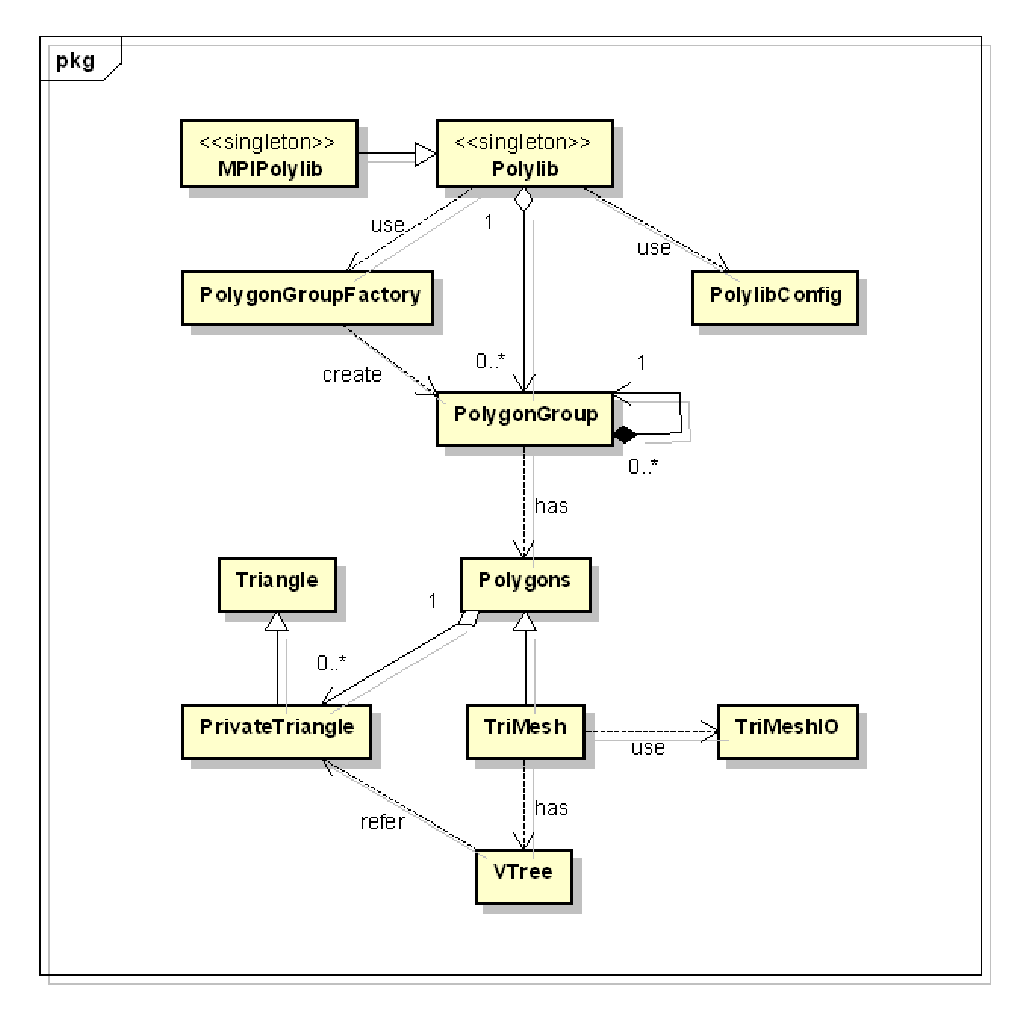
\includegraphics[width=12cm]{clip000.eps}
 \caption{主要クラス図}
\end{figure}

各クラスの説明は表\ref{tbl:classes}の通りです.

\pagebreak

\begin{table}[htbp]
 \begin{tabular}{|l|p{32em}|} \hline
 クラス名 & 概要 \\\hline
 \hline
 \multicolumn{1}{|l|}{Polylib} & 単一プロセス版のPolylib本体です.本クラス内部にポリゴングループ階層構造,三角形ポリゴン情報を保持します. \\
 \multicolumn{1}{|l|}{} & 本クラスはsingletonクラスであり,1プロセス内に1インスタンスのみ存在します. \\\hline
 MPIPolylib & MPI版のPolylib本体です.Polylibクラスを継承しており,各メソッドは並列処理を前提とした内容にオーバーライドされています. \\\hline
 PolylibConfig & Polylib初期化ファイルをload/saveするためのユーティリティクラスです. \\\hline
 PolygonGroup & 三角形ポリゴン集合をグルーピングして管理するためのクラスです.ポリゴングループ同士の階層的な包含関係も表現します.STLファイルから読み込んだ三角形ポリゴン集合を本クラスの属性であるPolygonsクラスインスタンスで管理します. \\\hline
 PolygonGroupFactory & Polylib初期化ファイルに記述されたポリゴングループ階層構造情報を元にPolygonGroupクラスとその継承クラスインスタンスを生成する処理を行うクラスです. \\\hline
 Polygons & 三角形ポリゴン情報を保持するコンテナクラスであり,ポリゴン検索のための検索メソッドを定義した抽象クラスです. \\\hline
 TriMesh & KD木による三角形ポリゴン検索アルゴリズムを実装したPolygonsクラスの導出クラスです. \\\hline
 TriMeshIO & STLファイルをload/saveするためのユーティリティクラスです. \\\hline
 Vtree & KD木データ構造クラスです. \\\hline
 Triangle & 三角形ポリゴンクラスです.3頂点座標,法線ベクトル,面積を保持します. \\\hline
 PrivateTriangle & Polylib内部で利用する三角形idなどを追加したTriangleクラスの導出クラスです. \\\hline
 \end{tabular}
 \caption{主要クラス一覧}
 \label{tbl:classes}
\end{table}

%
\section{データ構造}

\subsection{ポリゴングループの管理構造}

ポリゴングループの保持・管理は,Polylibクラスのメンバ変数である,std::vector$<$PolygonGroup$>$ m\_pg\_list
で行います.このvectorコンテナはポリゴングループ階層構造の最上位のPolygonGroupインスタンスを保持します.
PolygonGroupクラスは,メンバ変数std::vector$<$PolygonGroup*$>$ m\_childrenにより,PolygonGroupインスタンス同士
の階層構造を保持します.

PolygonGroupは複数の子要素を持つことができますが,親要素は最大で1つです.(親要素数がゼロならば最上位
のPolygonGroupです)また,階層構造最下位のPolygonGroupのみ,STLファイルから読み込んだ三角形ポリゴン情報
を保持します.

これらの階層構造については,ユーザが作成するPolylib初期化ファイルに記述されており,Polylibは初期化処理時
にこのファイルを読み込むことで,グループ階層構造,およびポリゴンデータをオンメモリに構築し,管理します.

\begin{figure}[H]
 \centering
 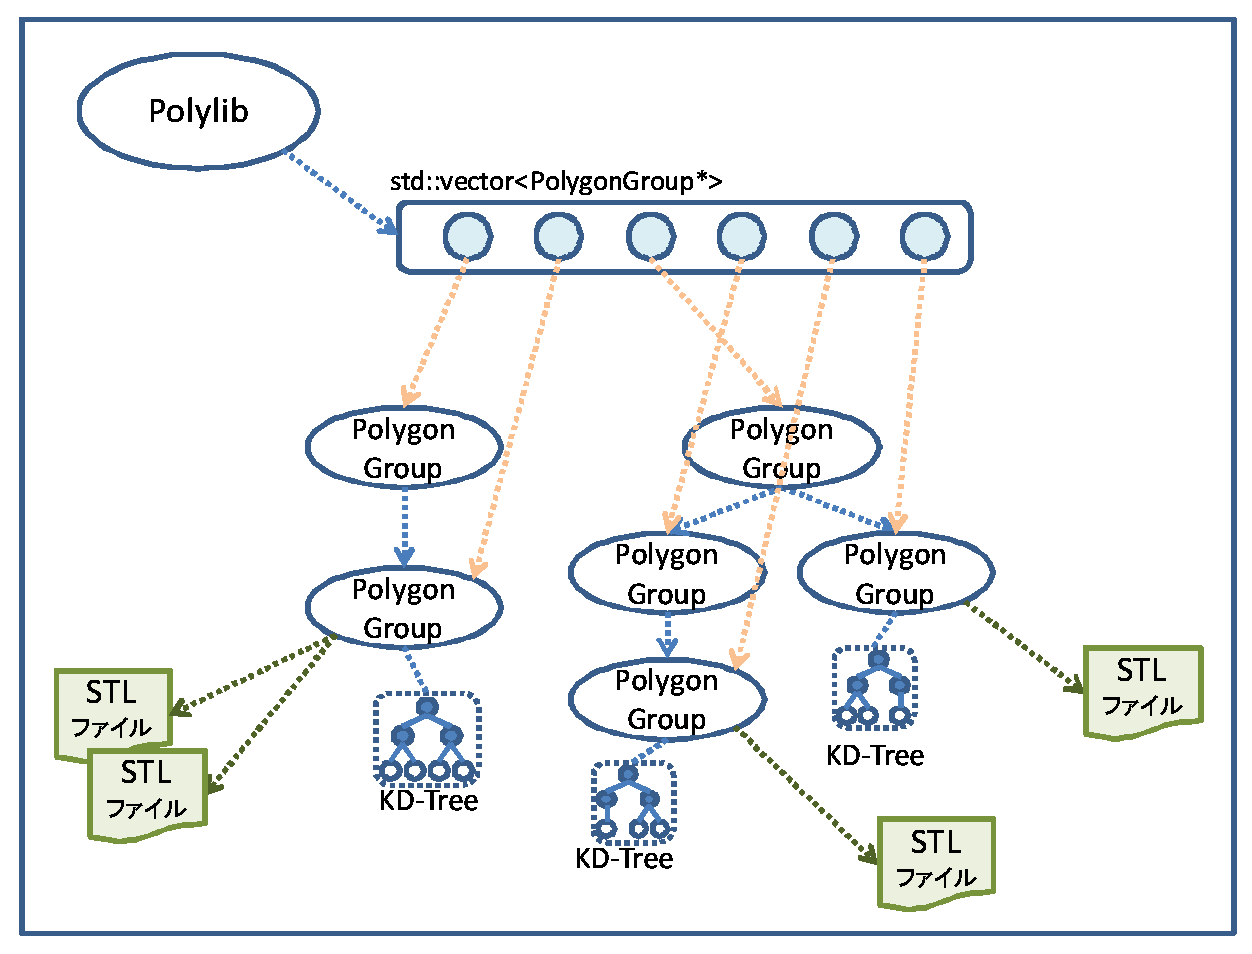
\includegraphics[width=10cm]{clip001.eps}
 \caption{ポリゴングループの管理構造}
\end{figure}

%
\subsection{ポリゴンデータの管理構造}

三角形ポリゴンの保持・管理は,Polygonsクラスのメンバ変数である,std::vector$<$PrivateTriangle*$>$ *m\_tri\_list
 で行います.このvectorコンテナには,STLファイルから読み込んだ三角形ポリゴン情報をPrivateTriangleクラス
インスタンスとして生成して登録します.

また,三角形ポリゴンを高速に検索するために,三角形ポリゴンのバウンディングボックスベースで包含判定を行う
KD-Tree構造を実装したTriMeshクラスをPolygonsクラスの導出クラスとして利用しています.KD木のリーフ要素で
ある三角形ポリゴン情報は,Polygons::m\_tri\_listコンテナに格納された各PrivateTriangleインスタンスへのポインタ
です.

Polylib::search()などのポリゴン検索メソッドは,このKD木を検索して得られたPrivateTriangle型ポインタの集合
をTriangle型ポインタにcastしてstd::vectorに詰めて返却します.検索メソッド呼び出し側では,返却結果の
std::vectorインスタンスを使用後にdeleteする必要がありますが,その要素であるTriangle型ポインタが指し示す
インスタンスを消去してはいけません.

\begin{figure}[H]
 \centering
 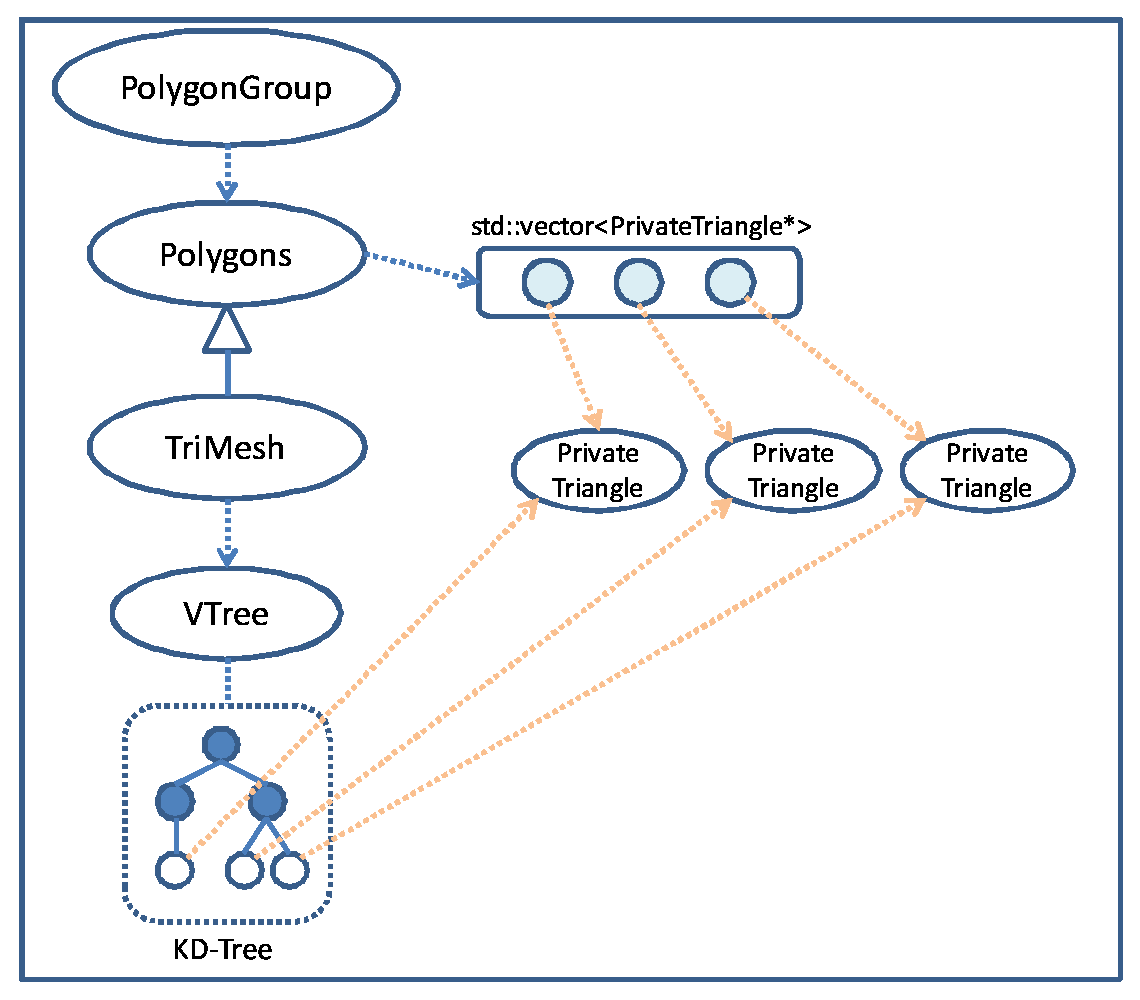
\includegraphics[width=8cm]{clip002.eps}
 \caption{ポリゴンデータの管理構造}
\end{figure}


%
\section{入力ファイル}

\subsection{Polylib初期化ファイル}

Polylib初期化ファイルは,Sphere初期化ファイルのユーザ定義パラメタ記述方式に準拠したXML形式のファイルです.
ElemタグとParamタグを利用して,ポリゴングループの階層構造を記述できます.ユーザ定義パラメタ記述方式の
基本的な考え方についてはSphereのマニュアルを参照してください.

Polylib初期化ファイルは,デフォルトではカレントディレクトリに存在する polylib\_config.xml を読み込みますが,
任意のファイル名をデータロードAPI引数で指定可能です.

記述例を以下に示します.

\begin{figure}[H]
 \centering
 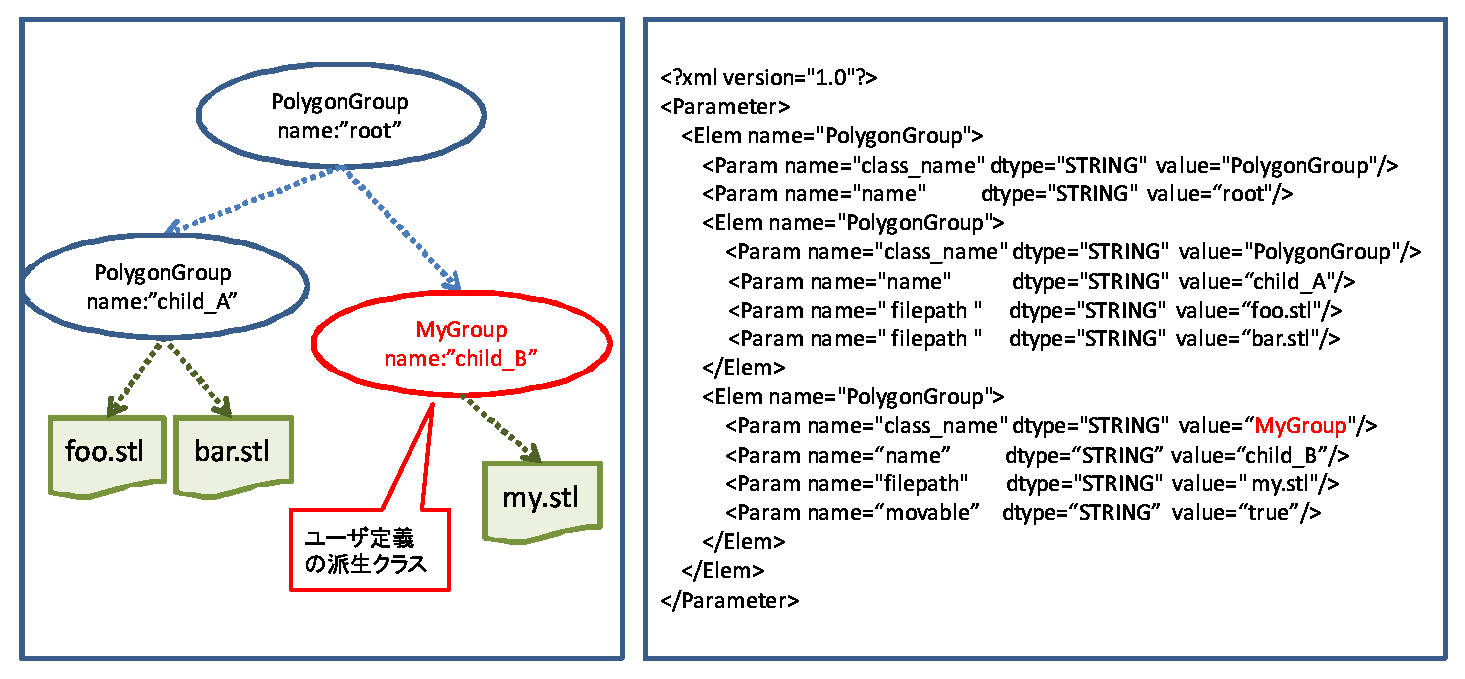
\includegraphics[width=16cm]{clip003.eps}\\
 \caption{初期化ファイルの例}
\end{figure}

各タグについて以下に説明します.

\begin{table}[htbp]
 \begin{tabular}{|l|p{34em}|} \hline
 タグ名 & 説明 \\\hline
 Parameter & Polylib初期化ファイルにおけるルートタグです.子要素としてElemタグを持つことができます. \\\hline
 Elem & ポリゴングループを表現します.子要素としてParamタグもしくはElemタグを持つことができます.name属性の値は必ず''PolygonGroup''でなければなりません. \\\hline
 Param & 各ポリゴングループの属性を表現します.子要素を持つことはできません. \\\hline
 \end{tabular}
 \caption{各タグの説明}
 \label{tbl:elem param}
\end{table}

\pagebreak

下表にParamタグの各属性値の書式を示します.

\begin{table}[htbp]
 \begin{tabular}{|l|l|p{34em}|} \hline
 name & dtype & 説明 \\\hline
 \hline
 class\_name & STRING & 生成するポリゴングループのクラス名.PolygonGroupクラスインスタンスを生成する場合は,''PolygonGroup''を指定.ユーザ定義の派生クラスインスタンスを生成する場合は,その派生クラスでオーバーライドしたメソッドget\_class\_name()が返す名称を指定する. \\\hline
 name & STRING & ポリゴングループの名称.名称は同じ階層内の同一レベルにおいて一意でなければならない. \\\hline
 \multicolumn{1}{|l|}{filepath} & \multicolumn{1}{l|}{STRING} & 当該ポリゴングループにひもづくSTLファイルのパス.カレントディレクトリからの相対パスまたは絶対パスで指定する. \\
 \multicolumn{1}{|l|}{} & \multicolumn{1}{l|}{} & 階層最下位のポリゴングループでのみ指定が可能. \\\hline
 \multicolumn{1}{|l|}{movable} & \multicolumn{1}{l|}{STRING} & 当該ポリゴングループがmove()メソッドにより移動するかどうかを指定する.valueには''ture''もしくは''false''を指定する. \\
 \multicolumn{1}{|l|}{} & \multicolumn{1}{l|}{} & 階層最下位のポリゴングループかつ,当該ポリゴングループがmove()メソッド実装済みのPolygonGroup派生クラスインスタンスの場合のみ指定が有効. \\\hline
 id & INT & ポリゴングループに付与可能なID番号.ID番号の重複は許される.省略可能で省略時は0が設定される.境界条件IDなどに利用されることを想定している. \\\hline
 \end{tabular}
 \caption{Paramタグの説明}
 \label{tbl:param tag}
\end{table}

上記Paramタグ属性値以外にも,ユーザ定義の属性値が指定可能です.ユーザ定義属性値の指定方法については,
後述のサンプルモデルによるチュートリアルを参照してください.

%
\subsection{STLファイル}
初期化ファイルで指定されたファイル名のSTLファイルを読み込みます.入力となるSTLファイルはアスキー形式
,バイナリ形式いずれでもかまいません.拡張子が"stl"であれば形式を自動判別して読み込みますが,拡張子が
"stla"であればアスキー形式として,"stlb"であればバイナリ形式として読み込みます.

%
\section{出力ファイル} \label{output_file}
本節では,Polylib::save()などのデータセーブ系APIで出力されたデータファイルについて説明します.

\subsection{Polylib初期化ファイル}

データセーブ時のポリゴングループの階層構造と,保存したSTLファイル名をpolylib初期化ファイル形式
で保存します.保存時のファイル命名規則は以下の通りです.

\begin{program}
	polylib_config_{ユーザ指定文字列}.xml
\end{program}

ユーザ指定文字列はデータセーブ系API引数で指定可能です.無指定の場合,保存時のタイムスタンプを
yyyymmddHHmmss形式で設定します.

%
\subsection{STLファイル}

データセーブ時のポリゴン情報を保存します.保存時のファイル命名規則は以下の通りです.

\begin{program}
	{ポリゴングループ名称フルパス}_{ユーザ指定文字列}.{stla|stlb}
\end{program}

ポリゴングループ名称フルパスとは,階層最上位のポリゴングループ名称から,当該グループ名称までを
'\_'でつなげたものです.
ユーザ指定文字列はデータセーブ系API引数で指定可能です.無指定の場合,保存時のタイムスタンプを
yyyymmddHHmmss形式で設定します.

ファイル拡張子はデータセーブ系APIで指定した保存ファイル形式に基づき設定されます.

MPIPolylibの場合,当該ポリゴングループについて自ランク内に保存すべき三角形ポリゴン情報が存在
しない場合はSTLファイルは出力されません.

なお,データロード時に指定したpolylib初期化ファイルにおいて,複数のSTLファイルを指定したポリゴン
グループについてデータセーブを行うと,ポリゴン情報は1つのSTLファイルに纏めて出力されます.

%
\subsection{三角形IDファイル}

MPIPolylib::save\_parallel()を利用したデータセーブ時にSTLファイル内の三角形ポリゴン並びに対応した三角形IDを保存します.

三角形IDとはMPIPolylibが管理する全三角形ポリゴン情報に対し,その三角形が所属するポリゴングループ内
で一意となるようなint型のID番号で,MPIPolylib内部でデータロード時に自動的に付与されます.

並列動作時に各ランク毎にデータセーブする場合,各計算領域ガイドセル部分の三角形情報は重複して保存
されるため,データを再ロードした際に重複三角形を判別するために三角形ID情報ファイルが必要となりま
す.

保存時のファイル命名規則は以下の通りです.

\begin{program}
	{ポリゴングループ名称フルパス}_{ユーザ指定文字列}.id
\end{program}

ポリゴングループ名称フルパスとは,階層最上位のポリゴングループ名称から,当該グループ名称まで
を'\_'でつなげたものです.

ユーザ指定文字列はデータセーブ系API引数で指定可能です.無指定の場合,保存時のタイムスタンプを
yyyymmddHHmmss形式で設定します.

なお,当該ポリゴングループについて自ランク内に保存すべき三角形ポリゴン情報が存在しない場合は三角形IDファイルは出力されません.


\chapter{API利用方法}
{\begin{abstract}
本章では,Polylibの主なAPIの利用方法を説明します.
\end{abstract}

% 
\graphicspath{{./fig_api/}}

%
\section{単一プロセス版の主なAPIの利用方法}

本節では単一プロセス版Polylibの主なAPI利用方法を,API呼び出し順に沿って説明します.

単一プロセス版PolylibのAPIを利用する手順は下図の通りです.

\begin{figure}[H]
 \centering
 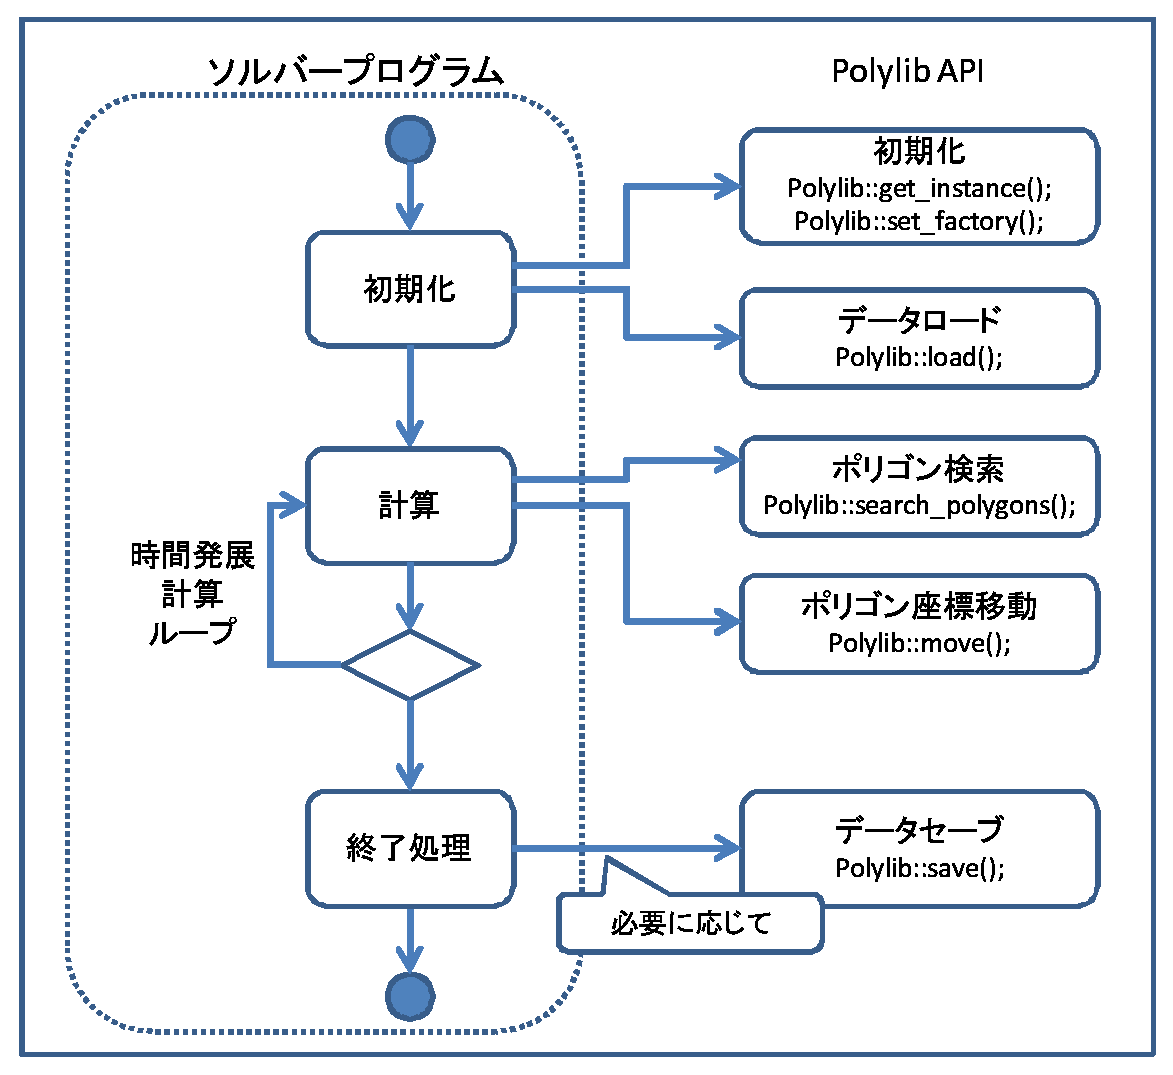
\includegraphics[width=12cm]{clip004.eps}\\
 \caption{API利用手順(単一プロセス版)}
\end{figure}

%
\subsection{初期化API}

%
\subsubsection{Polylibインスタンスの生成}
 \\

\begin{program}
	static Polylib* Polylib::get_instance();
\end{program}

Polylibはsingletonクラスのため,ユーザプログラム中からPolylibインスタンスを明示的に生成する
必要はありません.StaticメソッドであるPolylib::get\_instance()を呼び出すことで,プロセス内唯一
のPolylibインスタンスが返却されます.

また,Polylib::get\_instance()により返却されたインスタンスをユーザプログラムで明示的に消去する
必要はありません.インスタンスはプロセス終了時に自動的に消去されます.

%
\subsubsection{PolygonGroup派生クラスインスタンス生成ファクトリークラスの設定}
 \\

\begin{program}
	void Polylib::set_factory(
		PolygonGroupFactory *factory
	);
\end{program}

ユーザが定義するPolylgonGroup派生クラスを利用する場合,その派生クラスインスタンスの生成方法を
記述したPolygonGroupFactory派生クラスインスタンスを,本メソッドを利用してPolylibに登録する必要
があります.

PolylgonGroup派生クラスを利用しないのであれば,本APIを呼び出す必要はありません.

PolygonGroup派生クラスの具体的な利用法については後述のチュートリアルを参照してください.

%
\subsection{データロードAPI}

\begin{program}
	POLYLIB_STAT Polylib::load(
		std::string config_name = "polylib_config.xml"
	);
\end{program}

引数config\_nameで指定されたPolylib初期化ファイルを読み込み,そこに記述された内容に基づきポリゴン
グループ階層構造をオンメモリに生成します.そして最下層ポリゴングループに指定されたSTLファイルを
読み込み,三角形ポリゴン情報のインスタンスの生成と,ポリゴン検索用KD木の生成を行います.

引数config\_name が指定されなかった場合,デフォルト初期化ファイル名である"polylib\_config.xml"を
カレントディレクトリから読み込みます.

%
\subsection{検索API} \label{search_api}

\begin{program}
	std::vector<Triangle*>* Polylib::search_polygons(
		std::string	group_name,
		Vec3f		min_pos,
		Vec3f		max_pos,
		Bool		every
	)const;
\end{program}

ポリゴングループ名group\_nameで指定されたグループ階層構造下から,位置ベクトルmin\_posとmax\_posにより
指定される矩形領域に含まれる三角形ポリゴンを検索します.

引数group\_nameはポリゴングループ名称フルパスで指定します.ポリゴングループ名称フルパスとは,階層
最上位のポリゴングループ名称から,当該グループ名称までを'/'でつなげたものです.たとえば,階層最上位
のポリゴングループ名が"group\_A"でその直下にある"group\_B"内のポリゴンを検索する場合,引数group\_nameに
指定する文字列は以下の通りです.

\begin{program}
	"group_A/group_B"
\end{program}

引数everyの指定方法は以下の通りです.

\begin{itemize}
 \item ture:	3頂点が全て指定領域内に含まれる三角形を検索
 \item false:	一部でも指定領域と交差する三角形を検索
\end{itemize}

返却されたstd::vectorインスタンスは,呼び出し側で消去する必要がありますが,その要素であるTriangle型
ポインタの指し示すTriangleインスタンスを消去してはいけません.

%
\subsection{ポリゴン座標移動API}

\begin{program}
	POLYLIB_STAT Polylib::move(PolylibMoveParams& param);
\end{program}

Polylib管理下にあるmoveメソッド実装済のPolygonGroup派生クラスに所属する三角形ポリゴンの座標を,move
メソッドに実装された座標移動関数に基づきその頂点座標を変更します.

引数paramは,PolygonGroup派生クラスmoveメソッドの引数に渡されます.PolylibMoveParamsクラス定義は以下
の通りです.

\begin{program}
	class PolylibMoveParams {
	public:
		int m_current_step;	/*現在の計算ステップ番号*/
		int m_next_step;	/*移動後の計算ステップ番号*/
		double m_delta_t;	/*1計算ステップあたりの時間変異*/
	};
\end{program}

moveメソッドの実装方法の実際については,後述のチュートリアルを参照してください.

%
\subsection{データセーブAPI} \label{datasave_api}

\begin{program}
	POLYLIB_STAT Polylib::save(
		std::string	*p_fname,
		std::string	format,
		std::string	extend = ""
	);
\end{program}

本API呼び出し時点でのグループ階層構造をPolylib初期化ファイル形式に,三角形ポリゴン情報を
STLファイルに出力します.

引数p\_fnameは出力引数で,p\_fname の指し示すstd::stringインスタンスに保存されたPolylib初期
化ファイル名が設定されます.

引数formatは,保存するSTLファイルの形式を指定します."stl\_a"の場合,アスキー形式で保存
します."stl\_b"の場合,バイナリ形式で保存します.

引数extendは,保存するファイル名に任意の文字列を付加します.ファイル名の書式については,
\ref{output_file}を参照してください.


\pagebreak

%
\section{MPI版の主なAPIの利用方法}

本節ではMPI版Polylibの主なAPI利用方法を,API呼び出し順に沿って説明します.

MPI版PolylibのAPIを利用する手順は下図の通りです.

\begin{figure}[H]
 \centering
 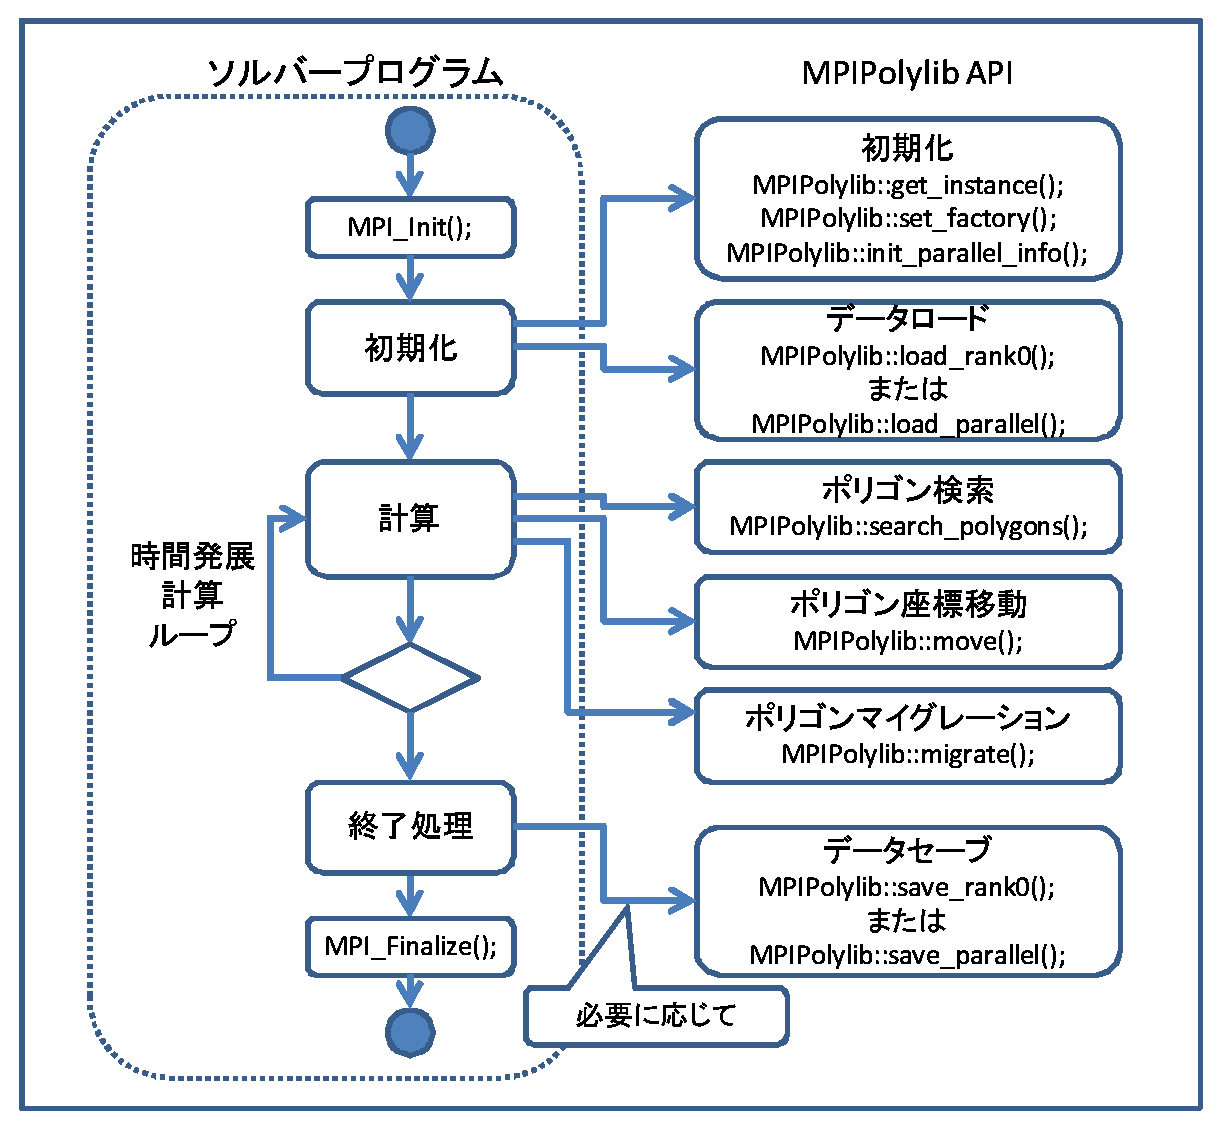
\includegraphics[width=12cm]{clip005.eps}
 \caption{API利用手順(MPI版)}
\end{figure}

%
\subsection{初期化API}

%
\subsubsection{MPIPolylibインスタンスの生成}
 \\

\begin{program}
	static MPIPolylib* MPIPolylib::get_instance();
\end{program}

MPIPolylibはPolylibクラスを継承し,MPI版機能を組み込んだクラスです.

Polylibクラス同様にsingletonクラスのため,ユーザプログラム中からMPIPolylibインスタンスを
明示的に生成する必要はありません.StaticメソッドであるMPIPolylib::get\_instance()を呼び出す
ことで,プロセス内唯一のMPIPolylibインスタンスが返却されます.

また,MPIPolylib::get\_instance()により返却されたインスタンスをユーザプログラムで明示的に
消去する必要はありません.インスタンスはプロセス終了時に自動的に消去されます.

%
\subsubsection{PolygonGroup派生クラスインスタンス生成ファクトリークラスの設定}
 \\

\begin{program}
	void MPIPolylib::set_factory(
		PolygonGroupFactory *factory
	);
\end{program}

ユーザが定義するPolylgonGroup派生クラスを利用する場合,その派生クラスインスタンスの生成方法
を記述したPolygonGroupFactory派生クラスインスタンスを,本メソッドを利用してPolylibに登録する
必要があります.

PolylgonGroup派生クラスを利用しないのであれば,本APIを呼び出す必要はありません.

PolygonGroup派生クラスの具体的な利用法については後述のチュートリアルを参照してください.

%
\subsubsection{並列計算情報の設定}
 \\

\begin{program}
	POLYLIB_STAT MPIPolylib::init_parallel_info(
		MPI_Comm     comm,
		float        bpos[3],
		unsigned int bbsize[3],
		unsigned int gcsize[3],
		float        dx[3]
	);
\end{program}

並列計算特有の値をMPIPolylibに設定します.各引数の意味は以下の通りです.

\begin{itemize}
 \item comm		MPIコミュニケータ
 \item bpos[3]	自ランクが受け持つ計算領域の基準座標
 \item bbsize[3]	自ランクが受け持つ計算領域のボクセル数
 \item gcsize[3]	自ランクが受け持つガイドセルのボクセル数
 \item dx[3]		ボクセル1辺の長さ
\end{itemize}

引数で設定された自ランク計算領域情報は,本API内部処理によりMPI通信により全ランクへ配信されます.

計算領域に関する各値の意味を下図に示します.

\begin{figure}[H]
 \centering
 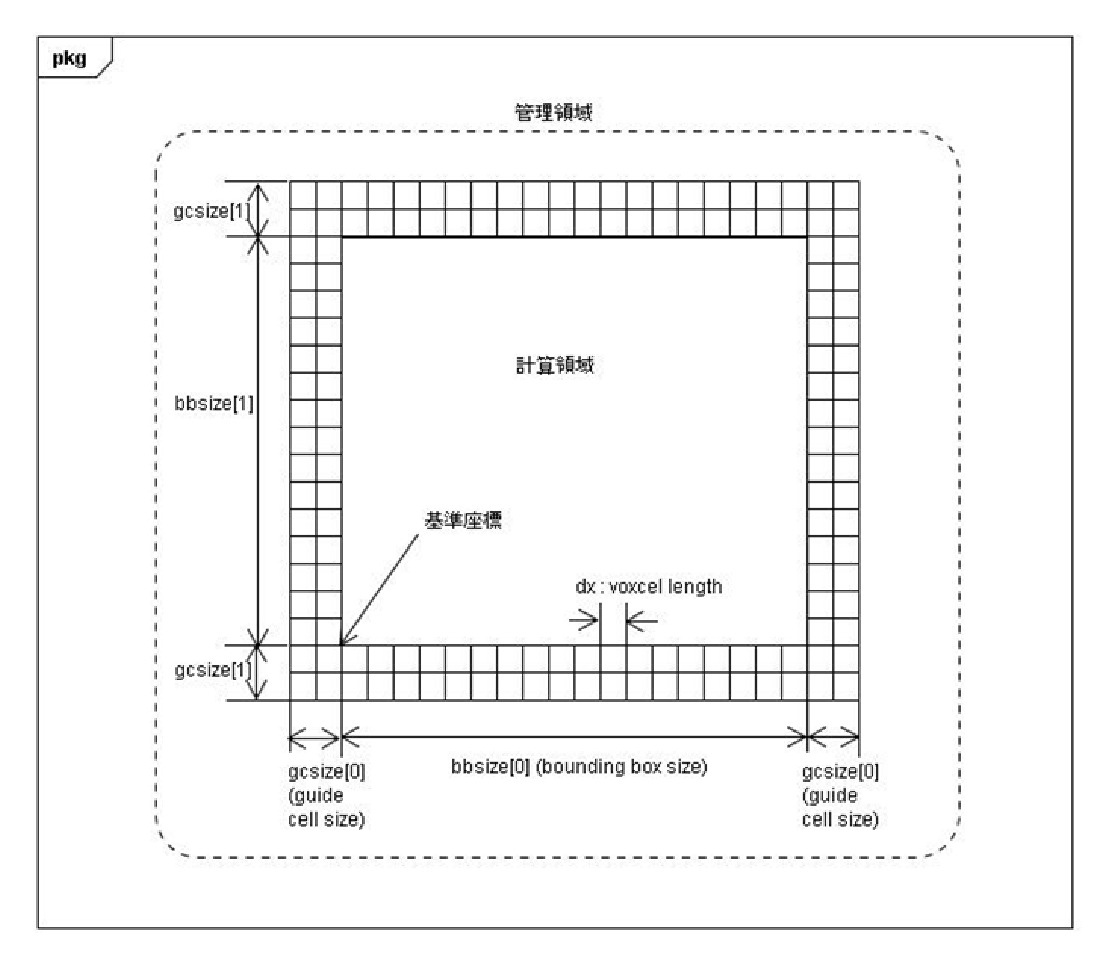
\includegraphics[scale=0.75]{clip006.eps}
 \caption{MPIPolylib::init\_parallel\_info() 各引数の意味}
\end{figure}


\subsection{データロードAPI}

\begin{program}
	POLYLIB_STAT MPIPolylib::load_rank0(
		std::string config_name = ""
	);

	POLYLIB_STAT MPIPolylib::load_parallel(
		std::string config_name = ""
		ID_FORMAT   id_format   = ID_BIN
	);
\end{program}

MPIPolylibでは2種類のデータロード系API があります.

MPIPolylib::load\_rank0は,rank0にてファイルを読み込み,他全ランクに対し,グループ階層情報と,
各ランクの担当領域ぶんのポリゴン情報をMPI通信にて配信します.

MPIPolylib::load\_paralellは,各ランクにてファイルを読み込みます.MPIPolylib::save\_parallelと
組み合わせて使用することで時間発展計算の中断/再開に対応しています.

いずれのAPIも,引数config\_nameで指定されたPolylib初期化ファイルを読み込み,そこに記述された
内容に基づきポリゴングループ階層構造をオンメモリに生成します.そして最下層ポリゴングループに
指定されたSTLファイルを読み込み,三角形ポリゴン情報のインスタンスの生成と,ポリゴン検索用KD木
の生成を行います.

引数config\_name が指定されなかった場合,デフォルト初期化ファイル名である"polylib\_config.xml"
をカレントディレクトリから読み込みます.

MPIPolylib::load\_paralellの引数id\_formatは,ロードする三角形IDファイルの形式を指定します.
未指定の場合,バイナリ形式の三角形IDファイルが存在するものとしてロード処理を行います.

%
\subsection{検索API}

\begin{program}
	std::vector<Triangle*>* Polylib::search_polygons(
		std::string	group_name,
		Vec3f		min_pos,
		Vec3f		max_pos,
		Bool		every
	)const;
\end{program}

MPIPolylibにおいても,検索APIは基底クラスPolylibのメソッドPolylib::search\_polygonsを利用します.

引数の説明は\ref{search_api}を参照してください.

\subsubsection{データセーブAPI}

\begin{program}
	POLYLIB_STAT MPIPolylib::save_rank0(
		std::string	*p_fname,
		std::string	format,
		std::string	extend = ""
	);

	POLYLIB_STAT MPIPolylib::save_parallel(
		std::string	*p_fname,
		std::string	format,
		std::string	extend = "",
		ID_FORMAT   id_format = ID_BIN
	);
\end{program}

MPIPolylibには2種類のデータセーブ系APIがあります.

MPIPolylib::save\_rank0は,本API呼び出し時点でのグループ階層情報とポリゴン情報をMPI通信
によりrank0に集計し,ファイルに出力します.

MPIPolylib::save\_parallelは,本API呼び出し時点でのグループ階層情報とポリゴン情報を各ランク
にてファイル出力します.

MPIPolylib::save\_paralellの引数id\_formatは,セーブする三角形IDファイルの形式を指定します.
未指定の場合,バイナリ形式でセーブ処理を行います.

各引数の意味については,\ref{datasave_api}を参照してください.

%
\subsection{ポリゴン座標移動API}

\begin{program}
	POLYLIB_STAT MPIPolylib::move(PolylibMoveParams& param);
\end{program}

MPIPolylib管理下にあるmoveメソッド実装済のPolygonGroup派生クラスに所属する三角形ポリゴンの
座標を,moveメソッドに実装された座標移動関数に基づきその頂点座標を変更します.

また,後述のメソッドMPIPolylib::migrate()の実行の前処理として,隣接ランク計算領域間をマイグレート
しそうな三角形ポリゴンにフラグを立てるなどの処理を行います.

moveメソッドを実装したPolygonGroup派生クラスインスタンスがMPIPolylib管理下にある場合,本メソッド
実行後にMPIPolylib::migrate()メソッドを実行する必要があります.

%
\subsection{ポリゴンマイグレーションAPI}

\begin{program}
	POLYLIB_STAT MPIPolylib::migrate();
\end{program}

前述のメソッドMPIPolylib::moveにより隣接ランク計算領域に移動した三角形ポリゴン情報を,
隣接ランク同士でMPI通信により送受信します.

\subsubsection{MPI版PolylibAPI利用の注意点}
 
\begin{itemize}
 \item MPIPolylibの内部では,MPIの初期化・終了処理は行いません.ソルバー側でMPI\_Init()およびMPI\_Finalize()を呼び出す必要があります.
 \item MPIPolylib::load\_parallel()は,MPIPolylib::save\_parallel()で保存されたファイル読み込みを前提としています.すなわち,読み込むべきPolylib初期化ファイルに記述されたグループ階層構造は全rankで一致しており,STLファイルは各ランク計算領域部分のポリゴン情報のみを保持しているものとします.また,三角形IDファイル形式についても,セーブ形式と同じ形式を指定してロードするものとします.
 \item MPIPolylibのAPIのうち,MPI通信を伴うAPIは全ランクで同時実行される必要があります.MPI通信を伴うAPIは以下の通りです.
 \begin{itemize}
  \item MPIPolylib::init\_parallel\_info();
  \item MPIPolylib::load\_rank0();
  \item MPIPolylib::save\_rank0();
  \item MPIPolylib::migrate();
 \end{itemize}
\end{itemize}


\pagebreak

%
\section{C言語用Polylib 主なAPI利用方法(単一プロセス版)}

本節ではC言語用の単一プロセス版Polylibの主なAPI利用方法を,API呼び出し順に沿って説明します.

C言語用単一プロセス版PolylibのAPIを利用する手順は下図の通りです.

\begin{figure}[H]
 \centering
 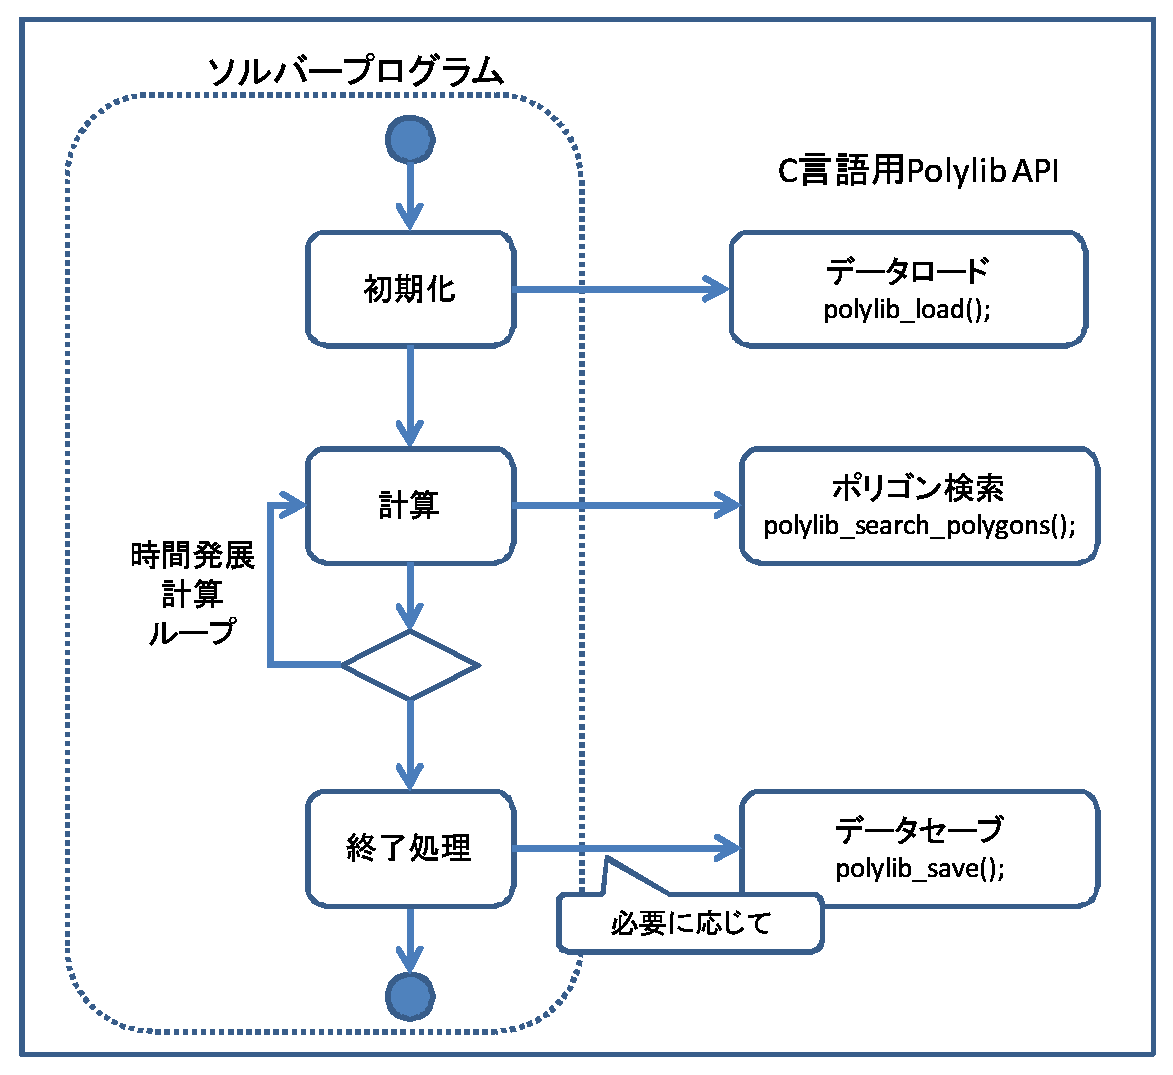
\includegraphics[width=12cm]{clip024.eps}\\
 \caption{API利用手順(C言語 単一プロセス版)}
\end{figure}

C言語用Polylibの各APIは基本的にC++版Polylibの各メソッドのラッピング関数として実現されています.
各APIの引数・返却値等はC言語向けに型変換されていること以外に違いはありません.

C言語用Polylibには,Polylib::move()相当の機能はありません.これは,Polylib::move()がクラスの
継承やメソッドの動的束縛など,オブジェクト指向プログラミングの仕組みを利用して実現されている
ためです.


\pagebreak

%
\section{C言語用Polylib 主なAPI利用方法(MPI版)}

本節ではC言語用のMPI版Polylibの主なAPI利用方法を,API呼び出し順に沿って説明します.

C言語用MPI版PolylibのAPIを利用する手順は下図の通りです.

\begin{figure}[H]
 \centering
 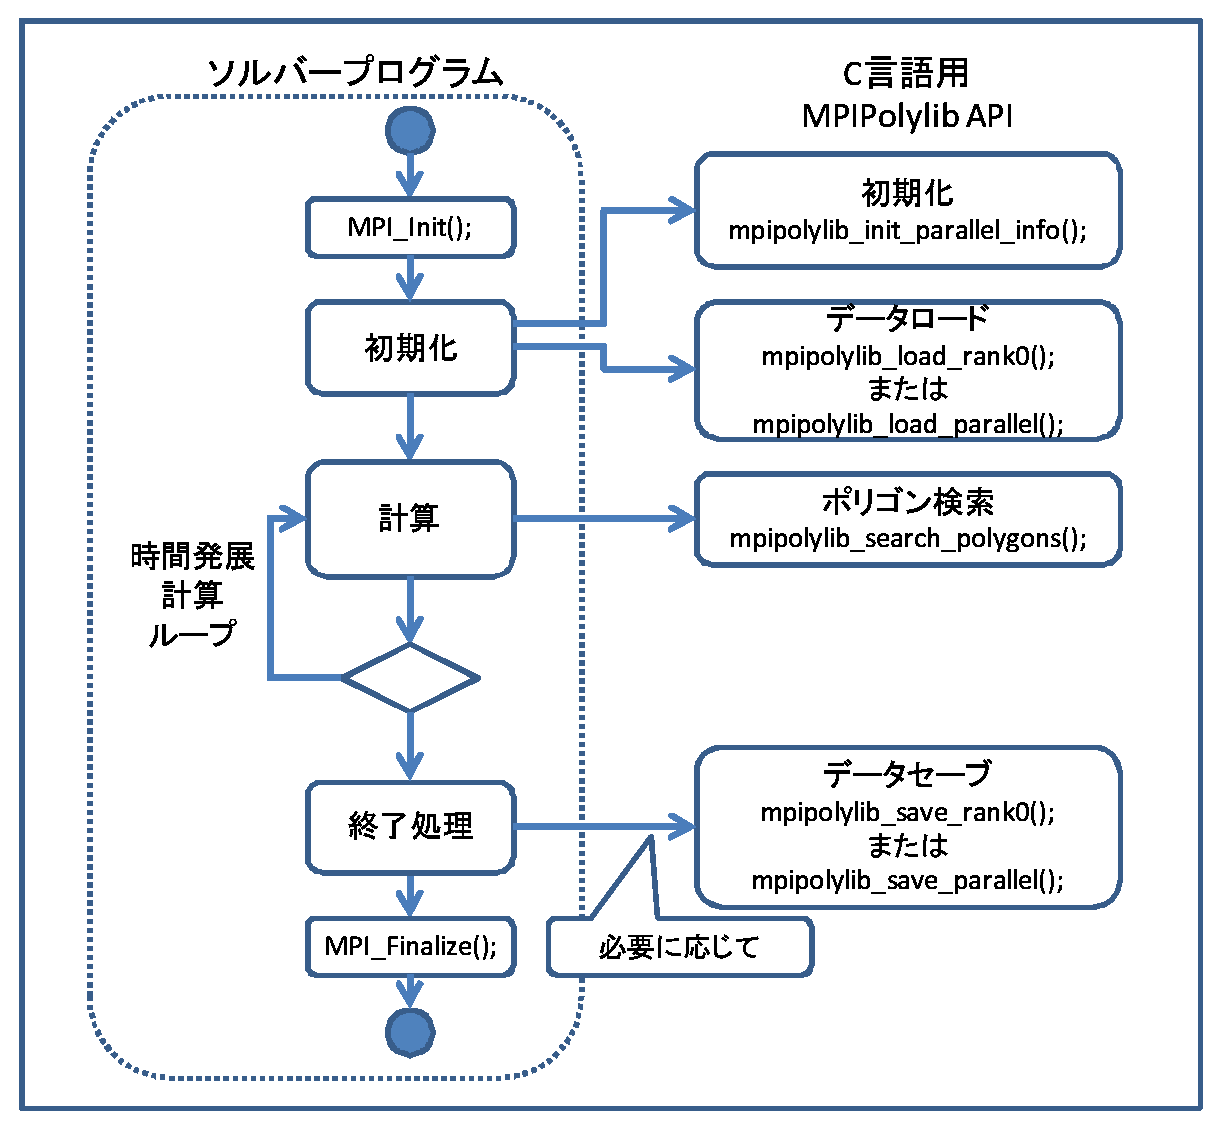
\includegraphics[width=12cm]{clip025.eps}\\
 \caption{API利用手順(C言語 MPI版)}
\end{figure}

C言語用MPIPolylibの各APIは基本的にC++版MPIPolylibの各メソッドのラッピング関数として実現されて
います.各APIの引数・返却値等はC言語向けに型変換されていること以外に違いはありません.

C言語用MPIPolylibには,MPIPolylib::move()やMPIPolylib::migrate()相当の機能はありません.これは,
これらの機能がクラスの継承やメソッドの動的束縛など,オブジェクト指向プログラミングの仕組みを
利用して実現されているためです.


\pagebreak

%
\section{動作確認用API}

本節ではPolylibおよびMPIPolylibの動作確認用APIについて説明します.これらのAPIはソルバー開発時
に利用するものであり,動作速度やメモリー消費量の点において非効率的ですので,通常のソルバー実行時
には利用しないでください.

%
\subsection{ポリゴングループ階層構造確認用API}

\begin{program}
	void Polylib::show_group_hierarchy(
		FILE	*fp = NULL
	);
\end{program}

Polylib管理下の全てのポリゴングループについて,その名称を階層レベルに従ったインデントをつけて
引数fpで指定されたファイルへ出力します.fpが未指定の場合は標準出力に出力します.

%
\subsection{ポリゴングループ情報確認用API}

\begin{program}
	void Polylib::show_group_info(std::string group_name);
\end{program}

指定された名称のポリゴングループについて,グループの情報と配下の三角形ポリゴン情報を標準出力に
出力します.

出力内容は以下の通り.

\begin{itemize}
 \item 親グループ名称
 \item 自身の名称
 \item STLファイル名
 \item 登録三角形数
 \item 各三角形の3頂点ベクトルの座標
 \item 法線ベクトルの座標
 \item 面積
\end{itemize}

%
\subsection{ポリゴン座標移動距離確認用API}

\begin{program}
	POLYLIB_STAT PolygonGroup::init_check_leaped();

	POLYLIB_STAT PolygonGroup::check_leaped(
		Vec3f	origin,
		Vec3f	cell_size
	);
\end{program}

PolygonGroup継承クラスでオーバーライドしたmove()メソッドにおいて,三角形ポリゴンの頂点座標
が隣接ボクセルより遠方へ移動したか否かをチェックするために利用するAPIです.

PolygonGroup::init\_check\_leaped()は,チェック処理の初期化関数です.move()メソッド内で,実際
に頂点移動処理を行う前に呼び出します.移動前の頂点座標を一時的に保存しますので,当該ポリゴン
グループの三角形ポリゴン数に応じてメモリを消費します.

PolygonGroup::check\_leaped()は,移動前後の頂点座標の距離を確認する関数です.move()メソッド内で,
頂点移動処理実行後に呼び出します.隣接ボクセルより遠方に移動した頂点については,標準エラー
出力にその三角形ID,移動前後の頂点座標情報を出力します.

出力例を以下に示します.

\begin{program}
PolygonGroup::check_leaped() Leaped Vertex Detected. GroupID:0 TriaID:2355
 before:(-16.0798 1093.99 -605.148) after:(-16.0798 1147.59 -496.047)
\end{program}

並列環境下で本APIを利用する場合,各ランクにおけるcheck\_leaped()の引数origin, cell\_sizeは,
MPIPolylib::get\_myproc()で取得できるParallelInfo構造体のメンバ変数m\_areaから取得することが
可能です.

なお,PolygonGroup::init\_check\_leaped()で確保された一時的メモリ領域は,PolygonGroup::check\_leaped()
を呼び出すと解放されます.

%
\subsection{メモリ消費量確認用API}

\begin{program}
	unsigned int Polylib::used_memory_size();

	unsigned int MPIPolylib::used_memory_size();
\end{program}

PolylibおよびMPIPolylibが確保しているメモリ量をbyte単位で返却します.

MPIPolylibの場合,本メソッドを呼び出したランクにおけるメモリ量が返されます.

報告されるメモリ消費量は概算です.ユーザ定義されたPolygonGroup派生クラスの拡張属性等のPolylib
フレームワーク外の消費メモリ利用については含まれません.

\pagebreak

%
\section{エラーコード}

Polylib内部でエラーが発生した場合に返却されるエラーコードPOLYLIB\_STAT型は,
include/common/PolylibStat.hに定義されています.
エラーコードの一覧を下表に示します.

\begin{table}[htbp]
\begin{tabular}{|l|l|} \hline
エラーコード & 意味 \\\hline
\hline
 PLSTAT\_OK & 処理成功 \\\hline
 PLSTAT\_NG & 一般的なエラー \\\hline
 PLSTAT\_INSTANCE\_EXISTED & Polylibインスタンスがすでに存在している \\\hline
 PLSTAT\_INSTANCE\_NOT\_EXIST & Polylibインスタンスが存在しない \\\hline
 PLSTAT\_STL\_IO\_ERROR & STLファイルIOエラー \\\hline
 PLSTAT\_UNKNOWN\_STL\_FORMAT & ファイル拡張子が.stla,.stlb,.stl以外 \\\hline
 PLSTAT\_FILE\_NOT\_SET & リーフグループにファイル名が未設定 \\\hline
 PLSTAT\_CONFIG\_ERROR & 定義ファイルでエラー発生 \\\hline
 PLSTAT\_GROUP\_NOT\_FOUND & グループ名がPolylibに未登録 \\\hline
 PLSTAT\_GROUP\_NAME\_EMPTY & グループ名が空である \\\hline
 PLSTAT\_GROUP\_NAME\_DUP & グループ名が重複している \\\hline
 PLSTAT\_MEMORY\_NOT\_ALLOC & メモリ確保に失敗した \\\hline
 PLSTAT\_POLYGON\_NOT\_EXIST & PolygonGroupにPolygonsが未設定 \\\hline
 PLSTAT\_TRIANGLE\_NOT\_EXIST & Polygonsに三角形リストが未設定 \\\hline
 PLSTAT\_NODE\_NOT\_FIND & KD木生成時に検索点が見つからなかった \\\hline
 PLSTAT\_ROOT\_NODE\_NOT\_EXIST & KD木のルートノードが存在しない \\\hline
 PLSTAT\_ARGUMENT\_NULL & 引数のメモリ確保が行われていない \\\hline
 PLSTAT\_MPI\_ERROR & MPI関数がエラーを戻した \\\hline
\end{tabular}
\caption{エラーコード一覧}
\label{tbl:error code}
\end{table}

\chapter{チュートリアル}
{\begin{abstract}
本章では,例題を用いたPolylibの使用法について説明します.
\end{abstract}
%

\graphicspath{{./fig_tutorial/}}

%
\section{サンプルモデルによるチュートリアル}
Polylibの利用方法を説明するために,以下のサンプルモデルを考えます.

各物体形状にはそれぞれ名前が付いており,時間発展計算の時刻ステップに応じて物体形状が移動する
物体についてはその移動計算式が分かっているものとします.

\begin{figure}[H]
 \centering
 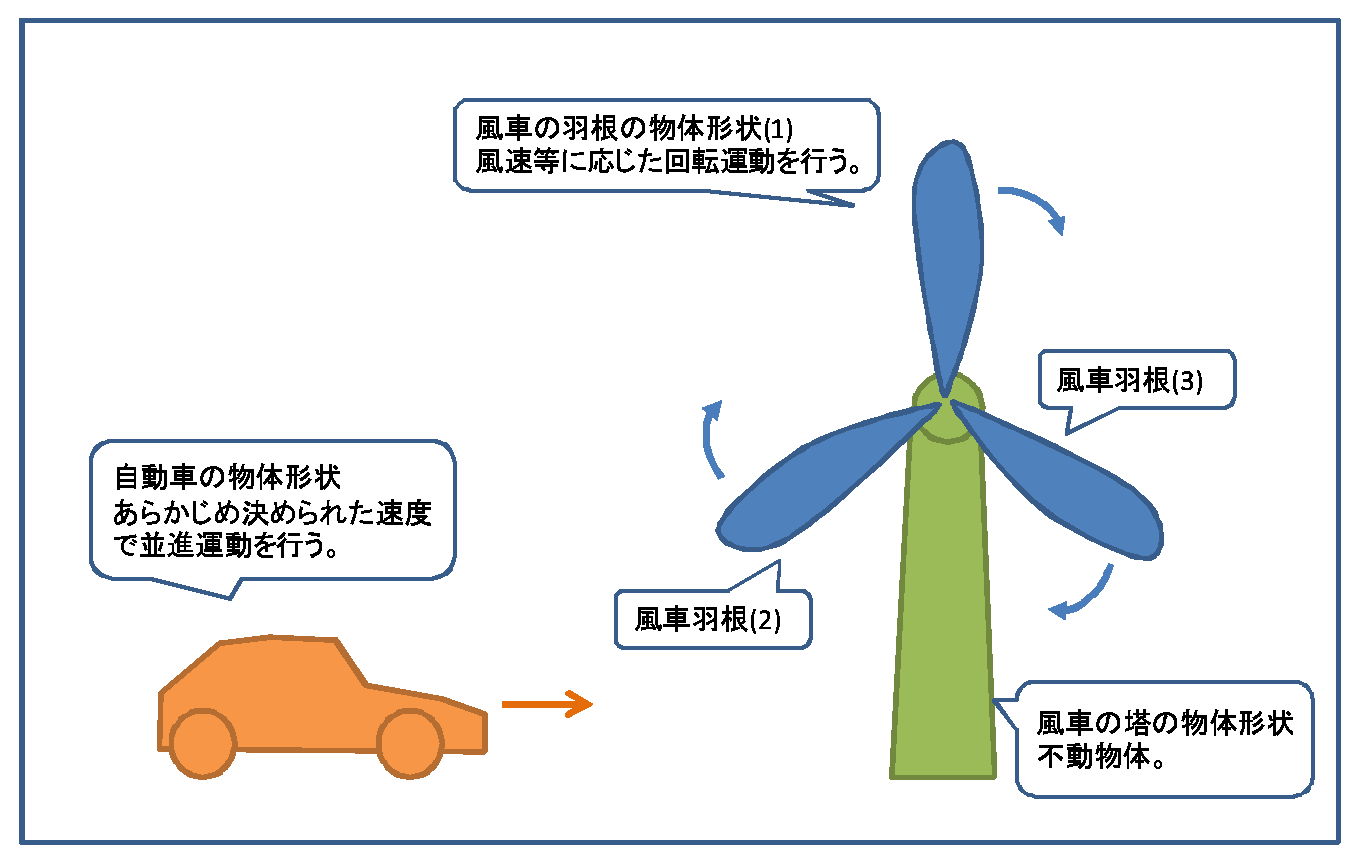
\includegraphics[scale=0.5]{clip007.eps}\\
 \caption{サンプルモデル}
\end{figure}


%
\subsection{物体形状のグルーピング}

Polylibでは物体形状ごとに,PolylgonGroupクラスインスタンスとして管理します.

PolylgonGroupクラスは,PolylgonGroupクラス同士による階層構造が表現可能です.

ライブラリユーザは,複数のPolygonGroupインスタンスを纏めて,概念的なグループを
表現することができます.

サンプルモデルについて,以下のようなグループ階層構造を定義することとします.

\begin{figure}[H]
 \centering
 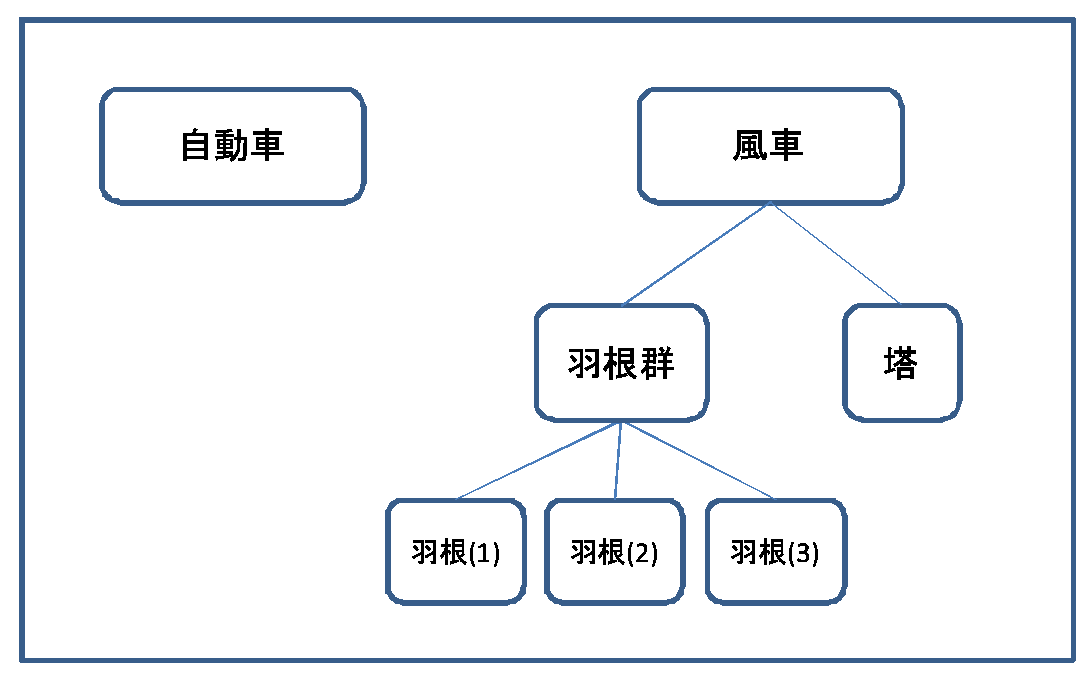
\includegraphics[scale=0.5]{clip008.eps}\\
 \caption{サンプルモデルのグループ階層構造}
\end{figure}

概念的なグループは,PolygonGroupクラスで表現することができます.特有の属性値を持
つグループや,物体形状が移動するようなグループは,PolygonGroupを派生させたユーザ
定義クラスで表現します.

サンプルモデルの風車の塔のような不動物体については,特に追加の属性などがなければ,
PolygonGroupクラスで表現します.

上記のグループ階層構造図をPolygonGroupクラスとユーザ定義の派生クラスを割り当てたも
のを下図に示します.(グループ名称もascii文字表現としました)

\begin{figure}[H]
 \centering
 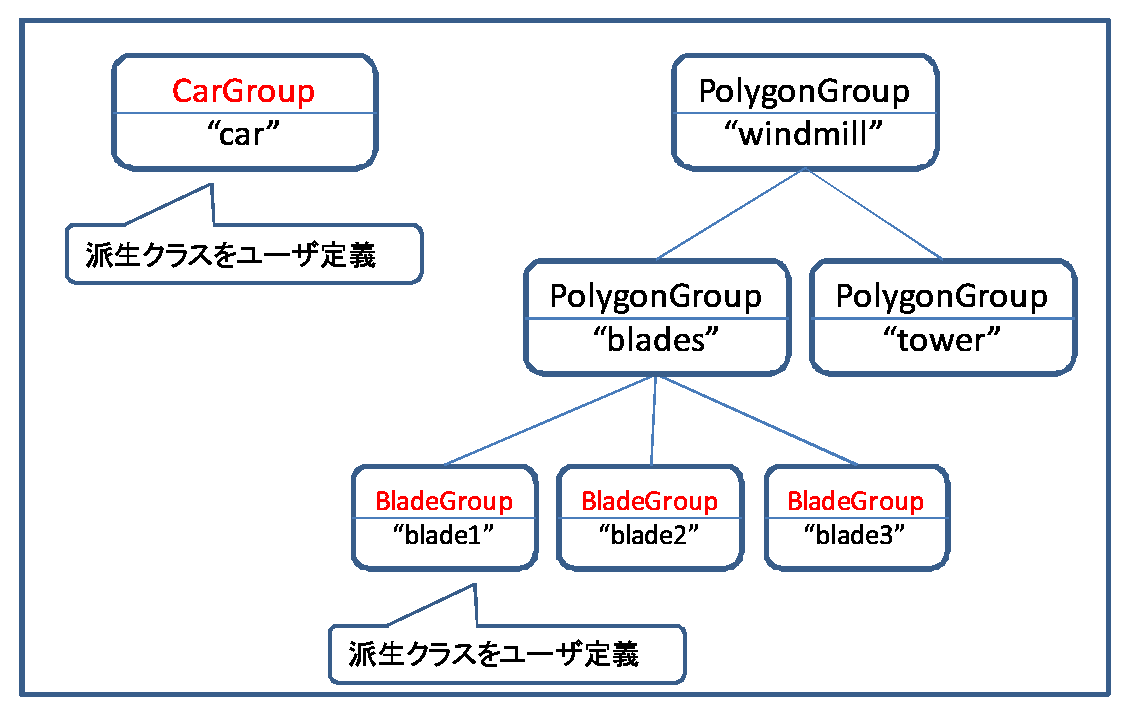
\includegraphics[scale=0.5]{clip009.eps}\\
 \caption{グループ階層構造図}
\end{figure}

%
\subsection{PolygonGroup派生クラスの定義}

ライブラリユーザは,PolygonGroupクラスを派生させた継承クラスを定義することができ
ます.

派生させることの意義は以下2点です.

\begin{itemize}
 \item 当該のポリゴングループに任意の属性値,メソッドを定義したいとき
 \item 当該のポリゴングループの座標移動計算式を定義したいとき
\end{itemize}

サンプルモデルでは,"car"が並行移動,"blade1","blade2","blade3"がそれぞれ回転移動
しますので,継承クラスを定義します.

\begin{figure}[H]
 \centering
 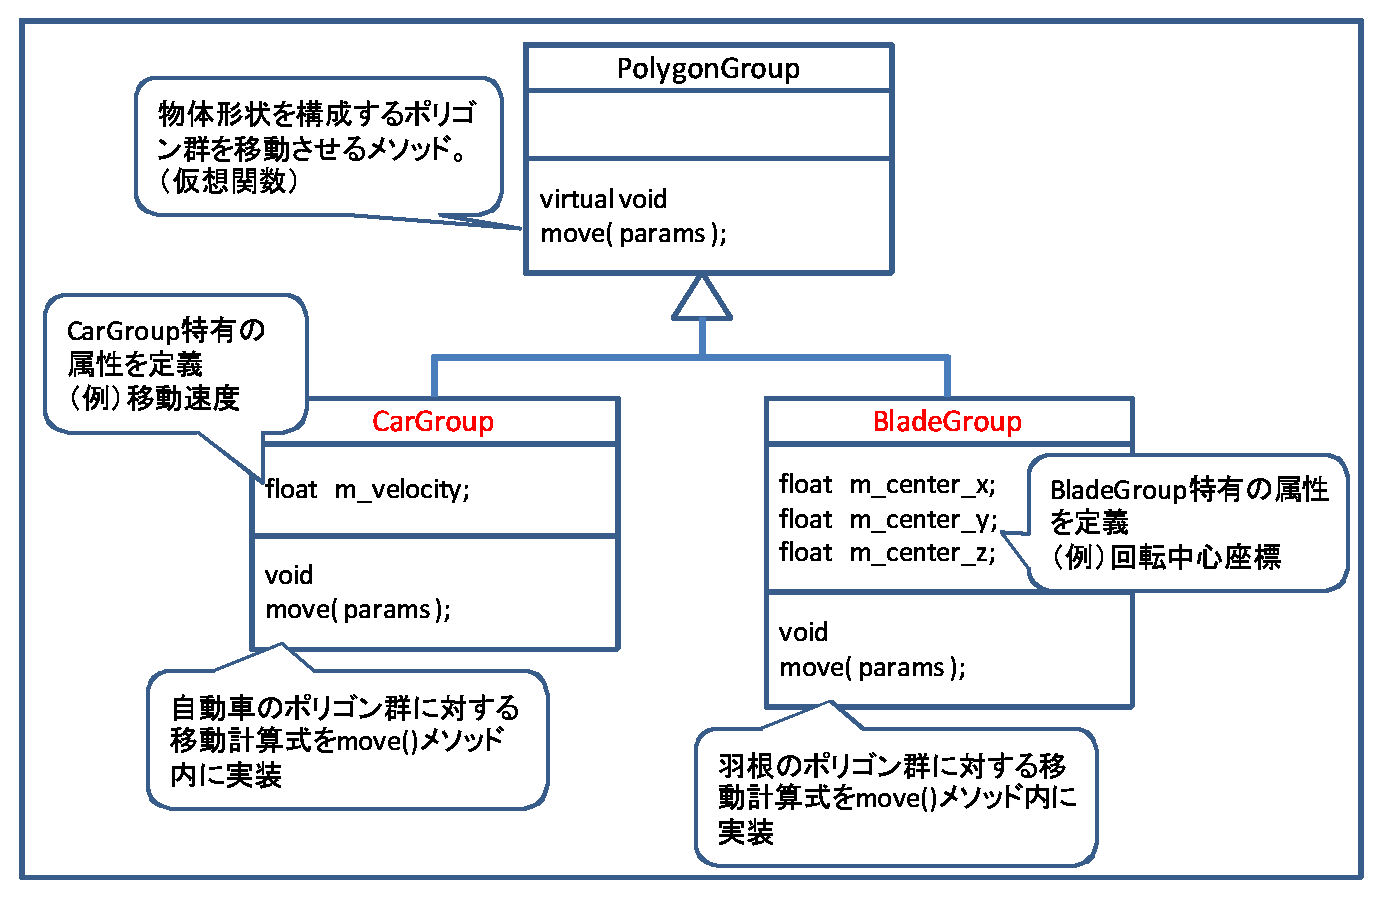
\includegraphics[width=13cm]{clip010.eps}\\
 \caption{PolygonGroupと派生クラス}
\end{figure}

派生クラスで追加した属性値は,整数,実数,文字列のいずれかであれば,グループ階層構
造構築メソッドPolygonGroup::build\_group\_tree()をオーバライドすることで,初期化ファイル
から値を取得することが可能です.CarGroupの追加属性float m\_velocityの値を取得する
CarGroup::build\_group\_tree()は以下のようになります.

\begin{program}
POLYLIB_STAT CarGroup::build_group_tree(
	Polylib			*polylib,
	PolygonGroup		*parent,
	const PolylibCfgElem	*elem
) {
	const PolylibCfgParam *att;

	// CarGroupクラスで追加定義した変数m_velocityに値を設定
	att = elem->first_param("velocity");
	if (att == NULL) {
		// エラー処理
		PL_ERROSH << "CarGroup::build_group_tree:[ERROR] velocity not found." 
			 << endl;
		return PLSTAT_CONFIG_ERROR;
	}
	m_velocity = att->get_real_data();

	// 基底クラスの属性値読み込み
	POLYLIB_STAT stat = PolygonGroup::build_group_tree(polylib, parent, elem);
	return stat;
}
\end{program}

また,追加属性をデータセーブ時にPolylib初期化ファイルに書き込むために,
PolygonGroup::mk\_param\_tag()メソッドをオーバーライドする必要があります.CarGroupの追加
属性float m\_velocityの値をPolylib初期化ファイルに保存するCarGroup:: mk\_param\_tag()は以下
のようになります.

\begin{program}
POLYLIB_STAT CarGroup::mk_param_tag(
	xmlNodePtr	elem,
	string		now,
	string		format,
	string		rank_no
){  
	POLYLIB_STAT	stat;

	// class_nameタグ作成
	stat = PolylibConfig::mk_param_tag(elem,
			PolygonGroup::ATT_NAME_CLASS, get_class_name().c_str());
	if (stat != PLSTAT_OK)	return PLSTAT_NG;

	// velocityタグ作成
	stat = PolylibConfig::mk_param_tag(elem, "velocity", m_velocity);
	if (stat != PLSTAT_OK)	return PLSTAT_NG;

	// 基底クラスが管理するタグ作成
	stat = PolygonGroup::mk_basic_tag(elem, now, format, rank_no);
	if (stat != PLSTAT_OK)	return PLSTAT_NG;

	return PLSTAT_OK;
}
\end{program}

ポリゴン群の座標移動計算式は,PolygonGroup::move()メソッドをオーバーライドして実装します.
たとえば並行移動を行うCarGroup::move()メソッドは以下のようになるでしょう.
\pagebreak
\begin{program}
POLYLIB_STAT
CarGroup::move(PolylibMoveParams&   params)
{
    // 引数チェック
    if (params.m_current_step == params.m_next_step)  return PLSTAT_OK;
    if (params.m_current_step > params.m_next_step)   return PLSTAT_NG;
    if (params.m_delta_t <= 0.0)                       return PLSTAT_NG;

    // 移動量
    // X軸方向に1stepあたりparams.m_delta_t × m_velocity だけ移動するものとする.
    float move_pos = (params.m_next_step - params.m_current_step) * 
                                         this->m_velocity * params.m_delta_t;

    // 三角形リストを取得
    std::vector<PrivateTriangle*>* tria_list = m_polygons->get_tri_list();
    std::vector<PrivateTriangle*>::iterator it;

    // 三角形リスト内の全ての三角形について頂点座標を更新
    for (it=tria_list->begin(); it!=tria_list->end(); it++) {
        PrivateTriangle *tria = (*it);
        Vec3f             *last_vtx = tria->get_vertex();
        Vec3f              moved_vtx[3];

        // X座標(t[0])のみ更新
        moved_vtx[0].t[0] = last_vtx[0].t[0] + move_pos;
        moved_vtx[1].t[0] = last_vtx[1].t[0] + move_pos;
        moved_vtx[2].t[0] = last_vtx[2].t[0] + move_pos;
        moved_vtx[0].t[1] = last_vtx[0].t[1];
        moved_vtx[1].t[1] = last_vtx[1].t[1];
        moved_vtx[2].t[1] = last_vtx[2].t[1];
        moved_vtx[0].t[2] = last_vtx[0].t[2];
        moved_vtx[1].t[2] = last_vtx[1].t[2];
        moved_vtx[2].t[2] = last_vtx[2].t[2];

        // 移動後の頂点座標を設定.法線ベクトルも再計算
        tria->set_vertexes( moved_vtx, true, false );
    }

    // 頂点座標が移動したことにより,KD木の再構築が必要.
    // 要再構築フラグを立てる.
    m_need_rebuild = true;

    return PLSTAT_OK;
}
\end{program}

実装したmove()メソッドで実際に三角形ポリゴン頂点座標が移動した場合,move()メソッド
内で,PolygonGroup::m\_need\_rebuildフラグをtrueにセットしなければならないことに注意
してください.このフラグをtureにしないとKD木の再構築が行われないため,
Polylib::search\_polygons()メソッドが正しい検索結果を返せなくなります.

また,PolygonGroup派生クラスでは,PolygonGroup::get\_class\_name()メソッドおよび
PolygonGroup::whoami()メソッドをオーバライドして実装し,システム一意なクラス名称を
返却するようにします.これは初期化ファイルに記述するクラス名称と一致させる必要が
あります.以下にCarGroupの場合の例を示します.

\begin{program}
static std::string CarGroup::get_class_name()
{
	return "CarGroup";
}

virtual std::string CarGroup::whoami()
{
	return get_class_name();
};
\end{program}

%
\subsection{PolygonGroupFactory派生クラスの定義}

サンプルモデルでは,CarGroupとBladeGroupの2種類の派生クラスがユーザ定義されました.


Polylibフレームワーク内部でこれら派生クラスインスタンスを生成するためには,生成
方法を記述した,PolygonGroupFactory派生クラスを定義する必要があります.

ここでは,MyGroupFactoryという名前の派生クラスを定義することとします.

\begin{figure}[H]
 \centering
 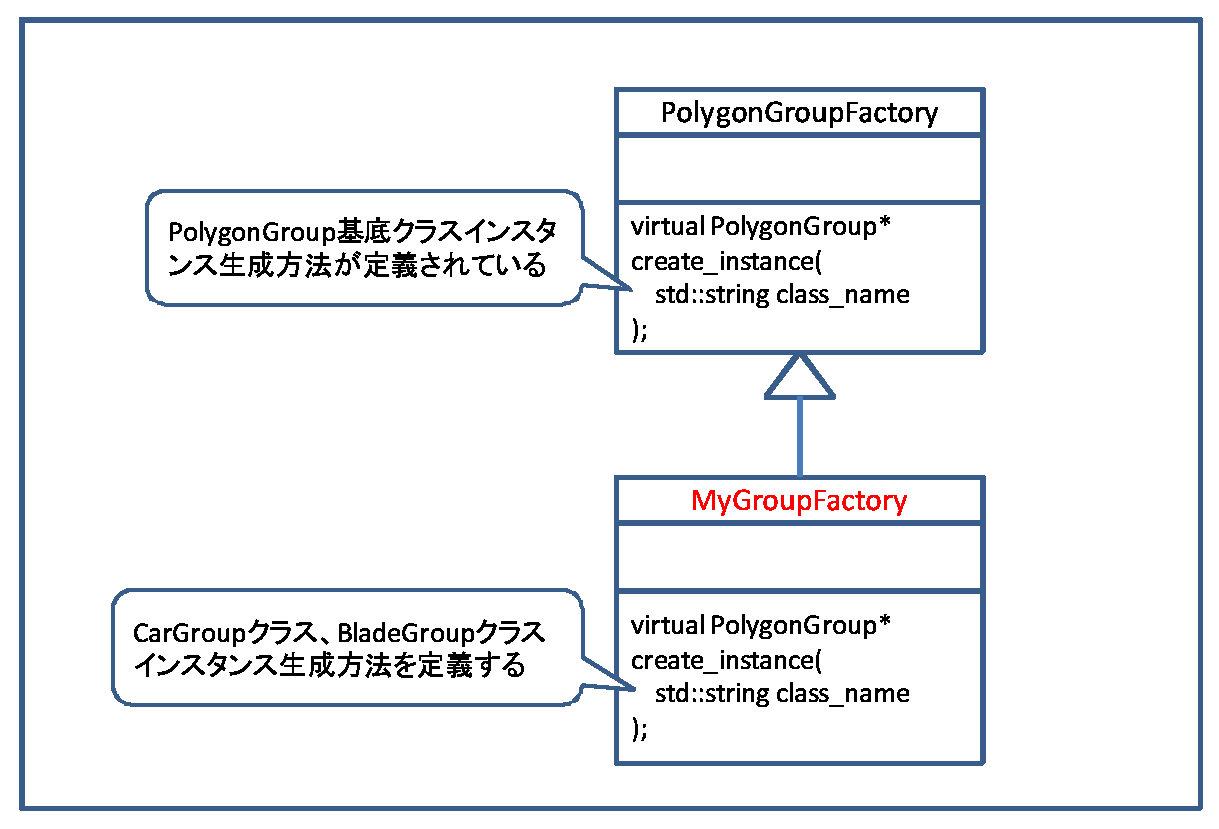
\includegraphics[width=11cm]{clip011.eps}\\
 \caption{PolygonGroupFactoryと派生クラス}
\end{figure}

Polylibには1つのPolygonGroupFactory派生クラスインスタンスしか登録できません.今回
のようにユーザ定義したPolygonGroup派生クラスが複数ある場合は,その全てのインスタンス
生成方法をMyGroupFactory::create\_instance()で実装します.以下にそのコード例を示します.

\begin{program}
PolygonGroup*
MyGroupFactory::create_instance( std::string  class_name )
{
    //---- class_nameに応じたインスタンスを生成
    // "CarGroup"の生成
    if (class_name == CarGroup::get_class_name()) {
         return new CarGroup();
    }
    // "BladeGroup"の生成
    if (class_name == BladeGroup::get_class_name()) {
         return new BladeGroup();
    }
    else {
         // 基底クラスのcreate_instanceに移譲
         return PolygonGroupFactory::create_instance(class_name);
    }
}
\end{program}

\pagebreak
%
\subsection{初期化ファイル}

サンプルモデルの初期化ファイルの内容を以下に示します.

\begin{program}
<?xml version="1.0"?>
<Parameter>
    <Elem name="PolygonGroup">
        <Param name="class_name" dtype="STRING" value="CarGroup"/>
        <Param name="name"       dtype="STRING" value="car"/>
        <Param name="filepath"   dtype="STRING" value="/foo/bar/car.stl"/>
        <Param name="movable"    dtype="STRING" value="true"/>
        <Param name="velocity"   dtype="REAL"   value="0.50"/>
    </Elem>
    <Elem name="PolygonGroup">
        <Param name="class_name" dtype="STRING" value="PolygonGroup"/>
        <Param name="name"       dtype="STRING" value="windomill"/>
        <Elem name="PolygonGroup">
            <Param name="class_name" dtype="STRING" value="PolygonGroup"/>
            <Param name="name"       dtype="STRING" value="blades"/>
            <Elem name="PolygonGroup">
                <Param name="class_name" dtype="STRING" value="BladeGroup"/>
                <Param name="name"       dtype="STRING" value="blade1"/>
                <Param name="filepath"   dtype="STRING" value="./blade1.stl"/>
                <Param name="movable"    dtype="STRING" value="true"/>
                <Param name="center_x"   dtype="REAL"   value="0.0"/>
                <Param name="center_y"   dtype="REAL"   value="123.45"/>
                <Param name="center_x"   dtype="REAL"   value="345.67"/>
            </Elem>
            <Elem name="PolygonGroup">
                <Param name="class_name" dtype="STRING" value="BladeGroup"/>
                <Param name="name"       dtype="STRING" value="blade2"/>
                <Param name="filepath"   dtype="STRING" value="./blade2.stl"/>
                <Param name="movable"    dtype="STRING" value="true"/>
                <Param name="center_x"   dtype="REAL"   value="0.0"/>
                <Param name="center_y"   dtype="REAL"   value="123.45"/>
                <Param name="center_x"   dtype="REAL"   value="345.67"/>
            </Elem>
            <Elem name="PolygonGroup">
                <Param name="class_name" dtype="STRING" value="BladeGroup"/>
                <Param name="name"       dtype="STRING" value="blade3"/>
                <Param name="filepath"   dtype="STRING" value="./blade3.stl"/>
                <Param name="movable"    dtype="STRING" value="true"/>
                <Param name="center_x"   dtype="REAL"   value="0.0"/>
                <Param name="center_y"   dtype="REAL"   value="123.45"/>
                <Param name="center_x"   dtype="REAL"   value="345.67"/>
            </Elem>
        </Elem>
        <Elem name="PolygonGroup">
            <Param name="class_name" dtype="STRING" value="PolygonGroup"/>
            <Param name="name"       dtype="STRING" value="tower"/>
            <Param name="filepath"   dtype="STRING" value="./tower.stl"/>
        </Elem>
    </Elem>
</Parameter>
\end{program}

\pagebreak

%
\subsection{メインプログラム}

以上のサンプルモデルを前提としたMPIPolylibを利用するメインプログラム例を以下に示します.

\begin{program}
#include <stdio>
#include "mpi.h"
#include "MPIPolylib.h"
#include "CarGroup.h"
#include "BladeGroup.h"
#include "MyGroupFactory.h"

using namespace std;
using namespace PolylibNS;

// 領域分割情報構造体定義
struct MyParallelInfo {
    float          bpos[3];  // 基準座標
    unsigned int bbsize[3];  // 計算領域ボクセル数
    unsigned int gcsize[3];  // ガイドセル領域ボクセル数
    float            dx[3];  // ボクセルサイズ
};

// 4並列を前提とした領域分割データ
static MyParallelInfo myParaInfos[4] = {
    {{-1100, -1800, -1800}, {18, 18, 18}, {1, 1, 1}, {100, 100, 100} },
    {{-1100,     0, -1800}, {18, 18, 18}, {1, 1, 1}, {100, 100, 100} },
    {{-1100, -1800,     0}, {18, 18, 18}, {1, 1, 1}, {100, 100, 100} },
    {{-1100,     0,     0}, {18, 18, 18}, {1, 1, 1}, {100, 100, 100} }
};

int main( int argc, char** argv )
{
    int             rank;
    unsigned int  step;
    POLYLIB_STAT  stat;
    PolylibMoveParams params;

    // MPI初期化
    MPI_Init( &argc, &argv );
    MPI_Comm_rank( MPI_COMM_WORLD, &rank );

    cout << "Starting program on rank:" << rank << endl;

    //---- MPIPolylibの初期化処理 -----
    // MPIPolylibインスタンス取得
    MPIPolylib *p_polylib = MPIPolylib::get_instance();

    // ユーザ定義ファクトリークラスを登録
    p_polylib->set_factory( new MyGroupFactory() );

    // 自PEの並列実行関連初期化情報の設定
    stat = p_polylib->init_parallel_info( MPI_COMM_WORLD,
                                    myParaInfos[rank].bpos,
                                    myParaInfos[rank].bbsize,
                                    myParaInfos[rank].gcsize,
                                    myParaInfos[rank].dx
                                );
    if( stat != PLSTAT_OK ) return -1;

    // データロード
    stat = p_polylib->load_rank0( "./polylib_config.xml" );
    if( stat != PLSTAT_OK ) return -1;

    // 時間発展計算ループ(100ステップ実行)
    for( step=0; i<100; step++ ){

        // 現在ステップでの計算実行…
        {
            // 必要なポリゴン情報を検索して取得
            vector<Triangle*>* trias =
                 p_polylib->search_polygons(/*検索条件を設定*/);

            // 検索結果ベクタの後始末
            delete trias;
        }

        // 次計算ステップへ進むためにポリゴン情報を更新
        // moveパラメタセットを設定
        PolylibMoveparams params;
        parmas.m_current_step = step;
        params.m_next_step     = step+1;
        params.m_delta_t       = 1.0;

        // move実行
        stat = p_polylib->move(params);
        if( stat != PLSTAT_OK ) return -1;

        // migrate実行
        stat = p_polylib->migrate();
        if( stat != PLSTAT_OK ) return -1;
    }

    // 各ランク毎にデータセーブ.STLはアスキー形式で出力.
    string fname;
    stat = p_polylib->save_parallel( &fname, "", "stl_a" );
    if( stat != PLSTAT_OK ) return -1;
    cout << "saved filename:" << fname << endl;

    // MPI終了処理
    MPI_Finalize();
    return 0;
}
\end{program}

\chapter{内部設計情報}
{\begin{abstract}
本節では,PolylibおよびMPIPolylibの内部設計について,UMLシーケンス図を用いて説明します.
\end{abstract}
%

\graphicspath{{./fig_design/}}

%
\section{Polylibクラス}

%
\subsection{Polylib::load()の内部処理シーケンス}

\begin{figure}[H]
 \centering
 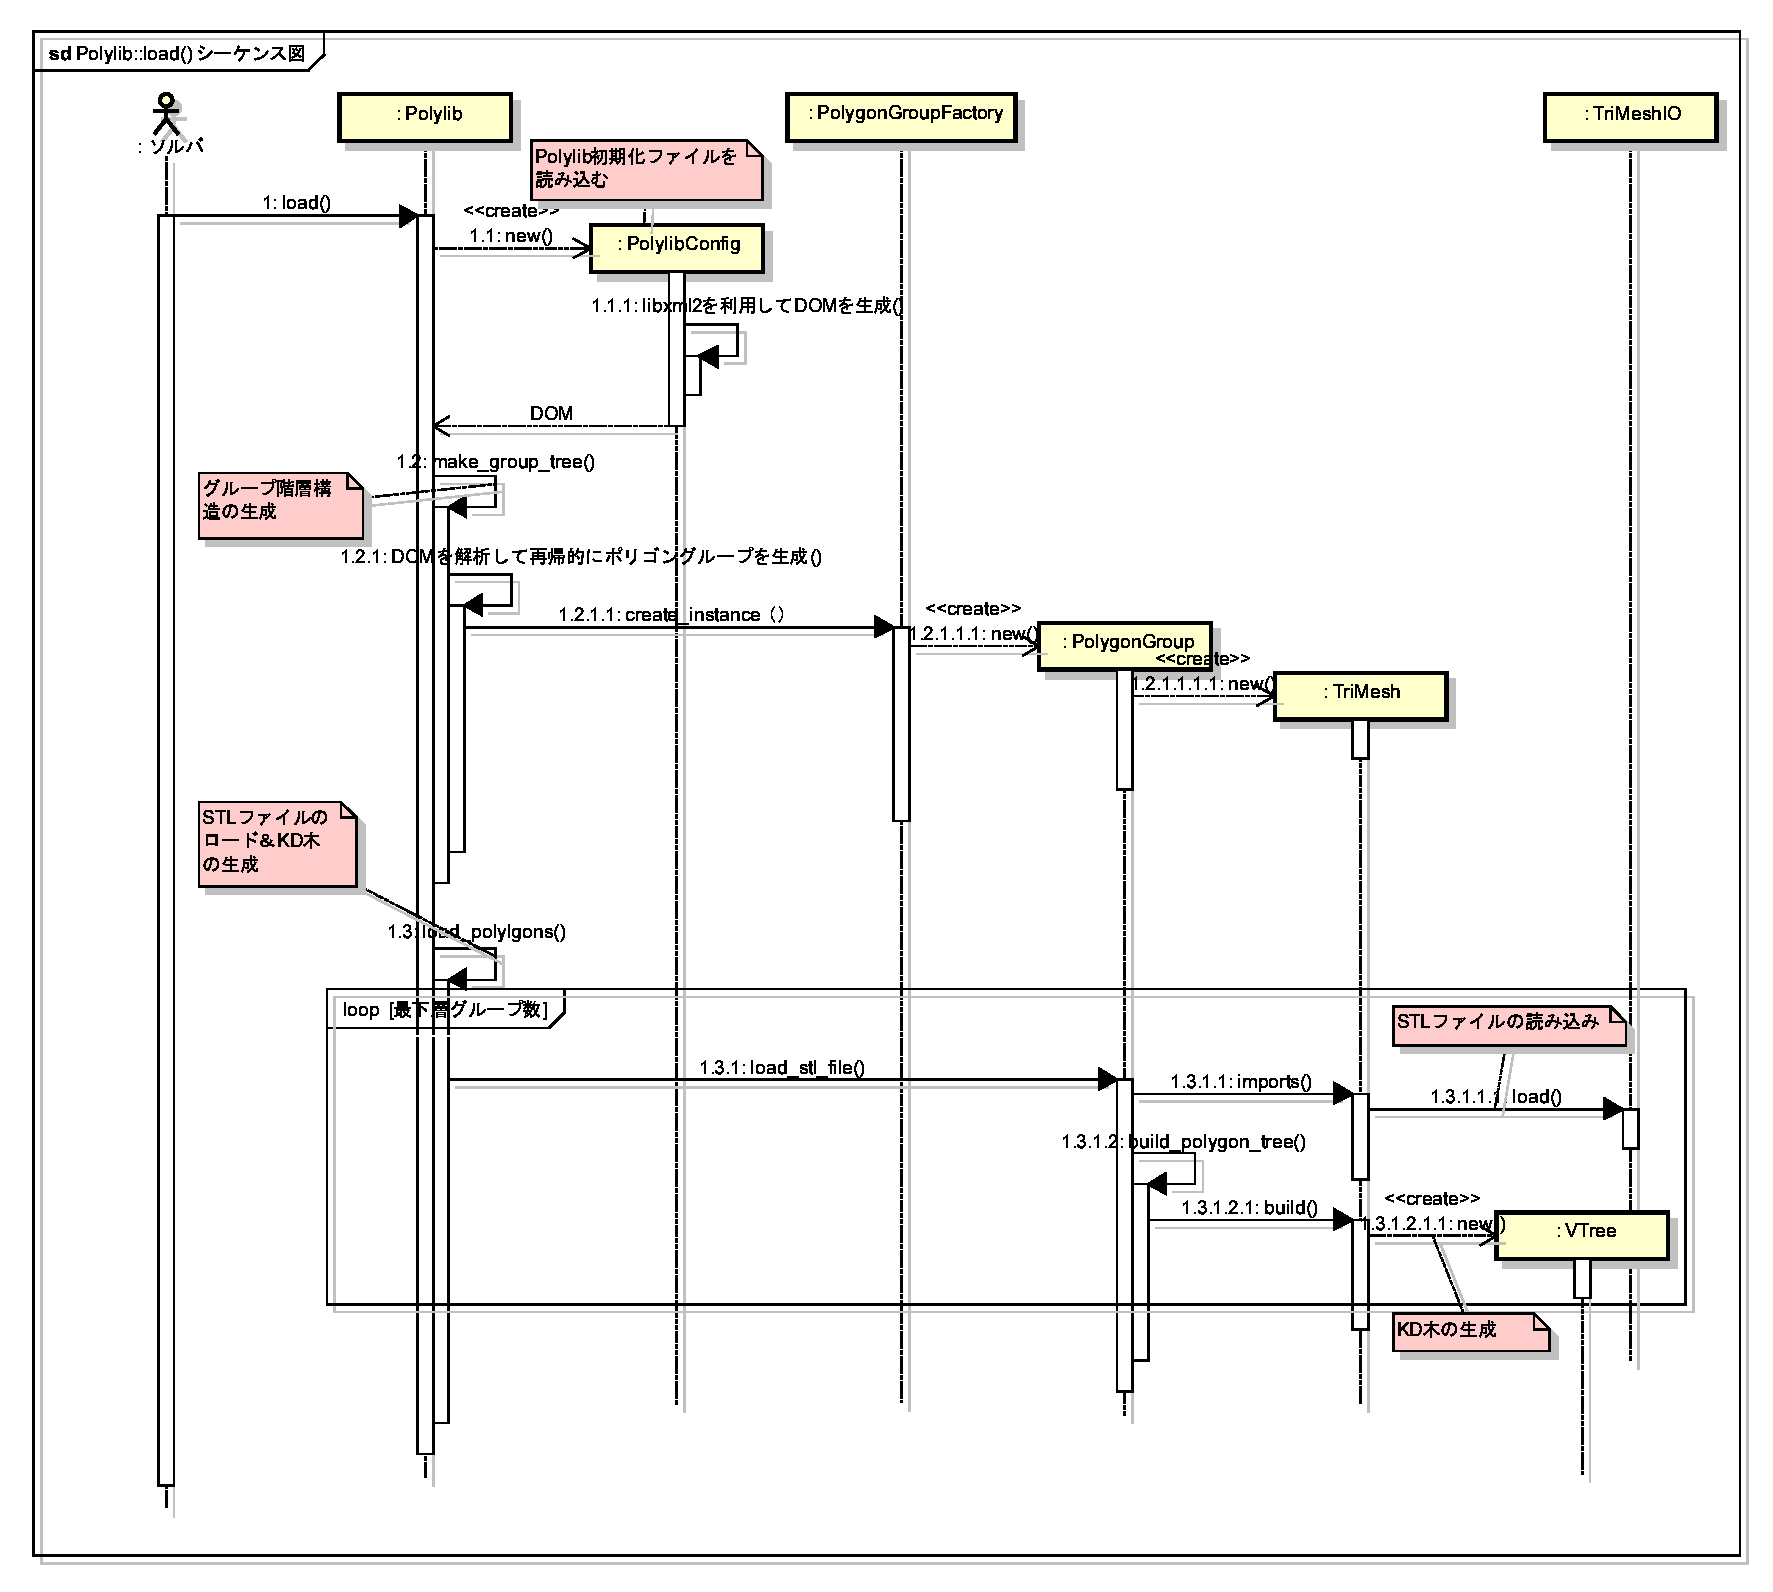
\includegraphics[width=16cm]{clip012.eps}
\end{figure}


\pagebreak
%
\subsection{Polylib::search\_polygons()の内部処理シーケンス}

\begin{figure}[H]
 \centering
 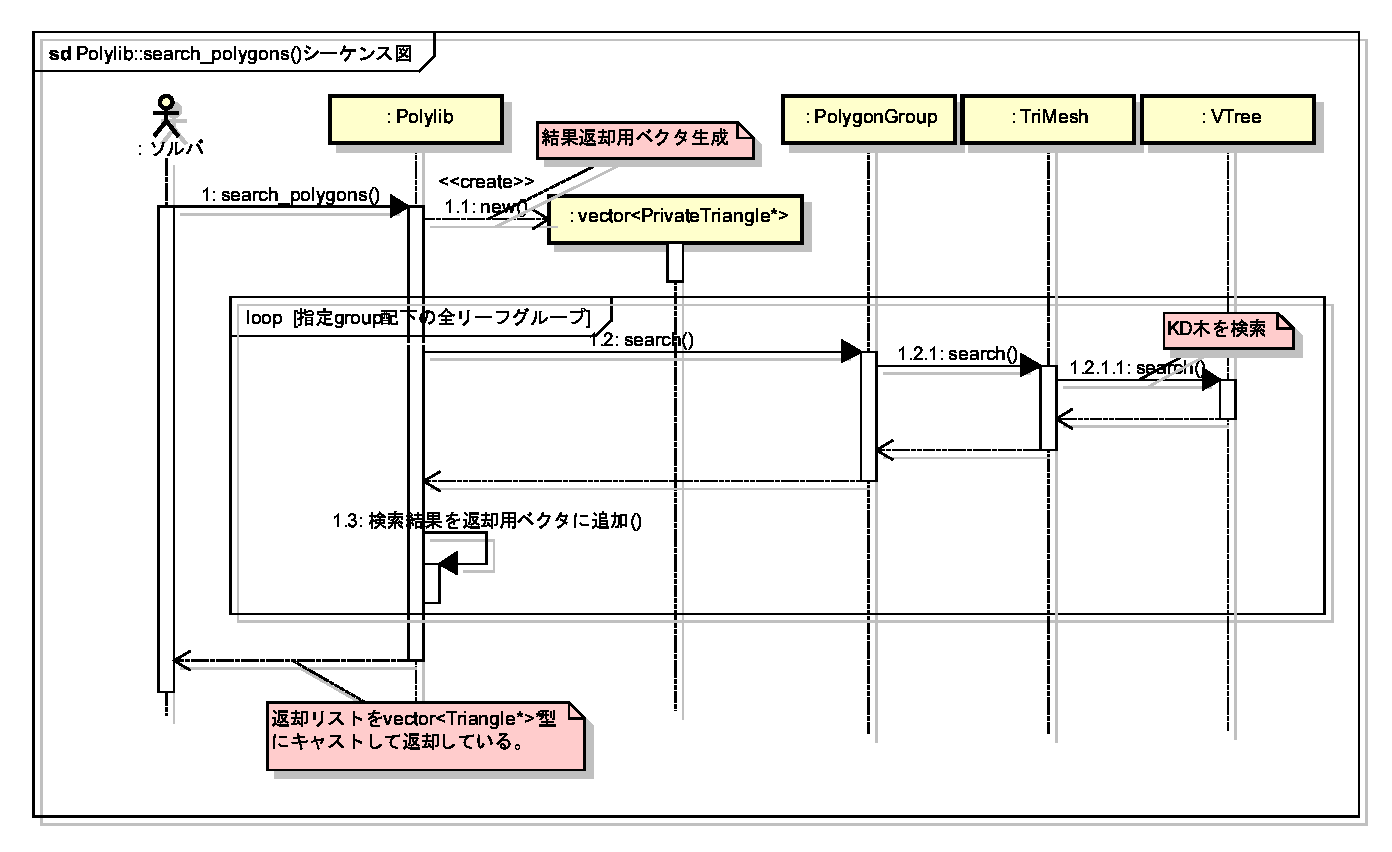
\includegraphics[width=15cm]{clip013.eps}
\end{figure}


%
\subsection{Polylib::move()の内部処理シーケンス}

\begin{figure}[H]
 \centering
 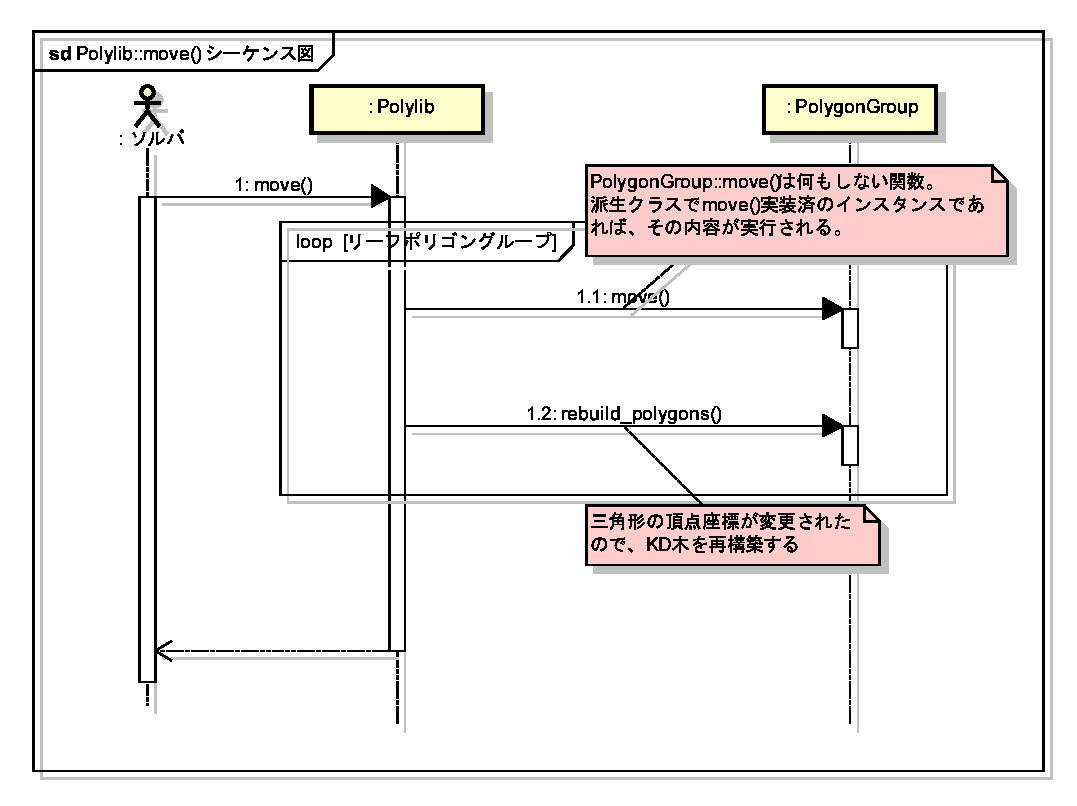
\includegraphics[width=12cm]{clip014.eps}
\end{figure}


\pagebreak
%
\subsection{Polylib::save()の内部処理シーケンス}

\begin{figure}[H]
 \centering
 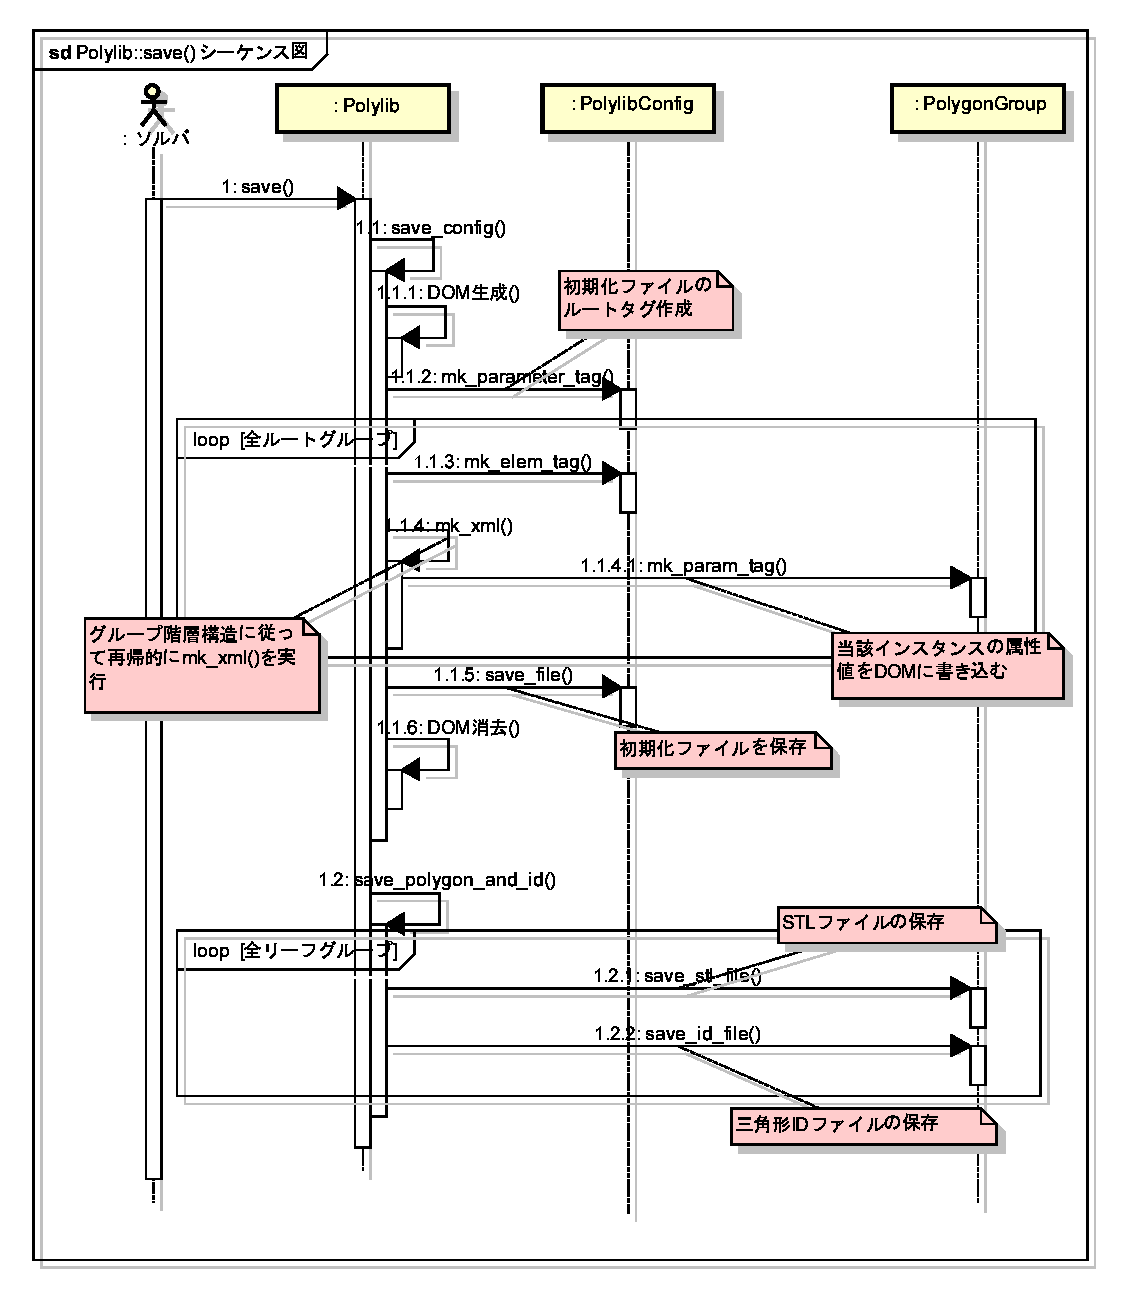
\includegraphics[width=15cm]{clip015.eps}
\end{figure}


\pagebreak
%
\section{MPIPolylibクラス}

%
\subsection{MPIPolylib::init\_parallel\_info()の内部処理シーケンス}

\begin{figure}[H]
 \centering
 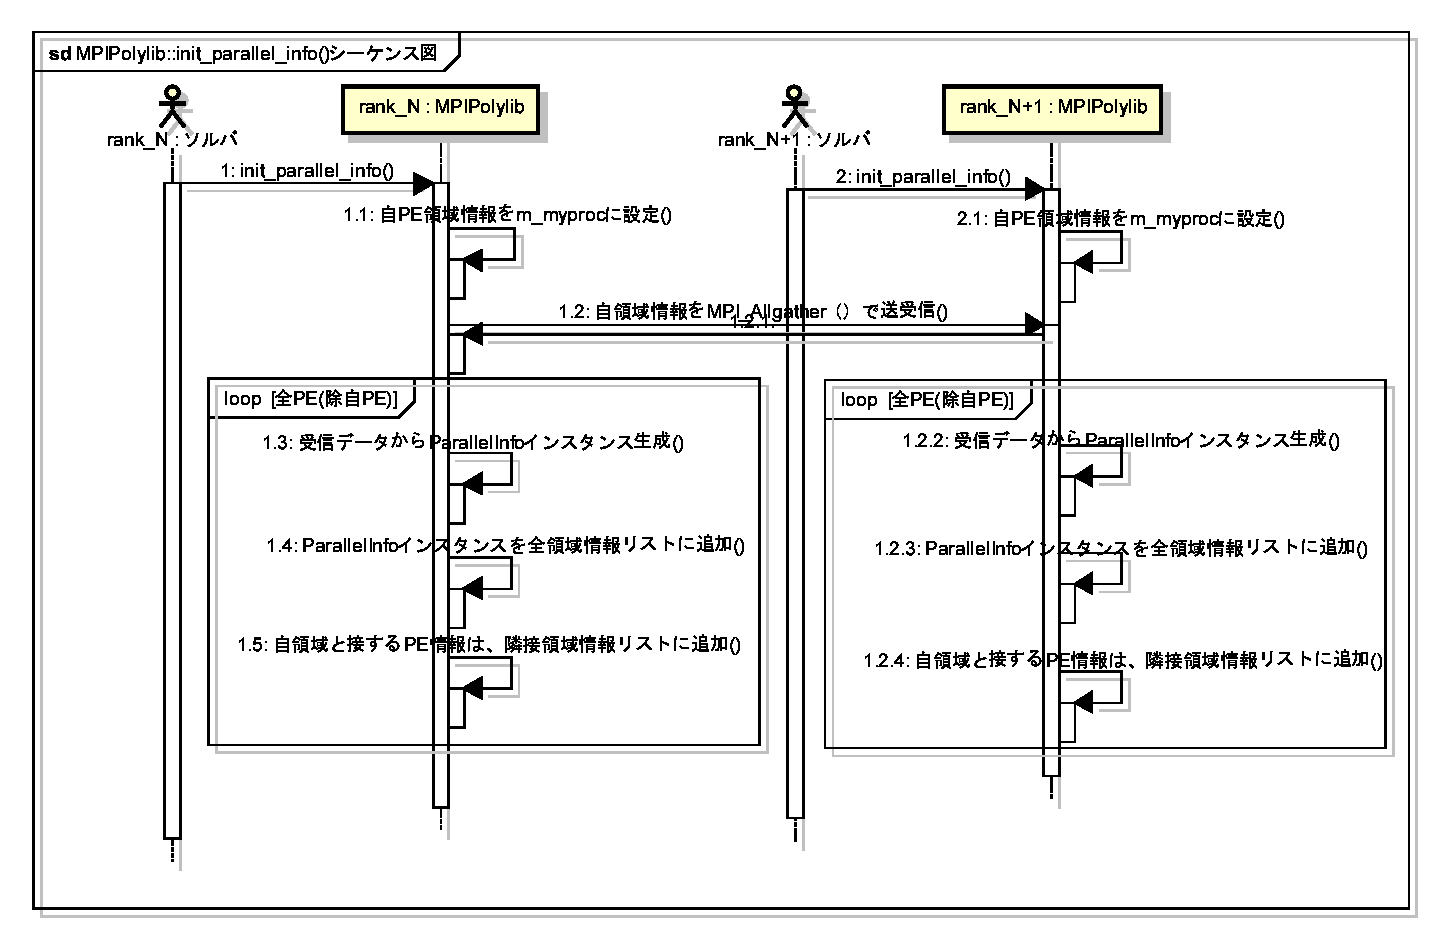
\includegraphics[width=16cm]{clip016.eps}
\end{figure}


\pagebreak
%
\subsection{MPIPolylib::load\_rank0()の内部処理シーケンス}

\begin{figure}[H]
 \centering
 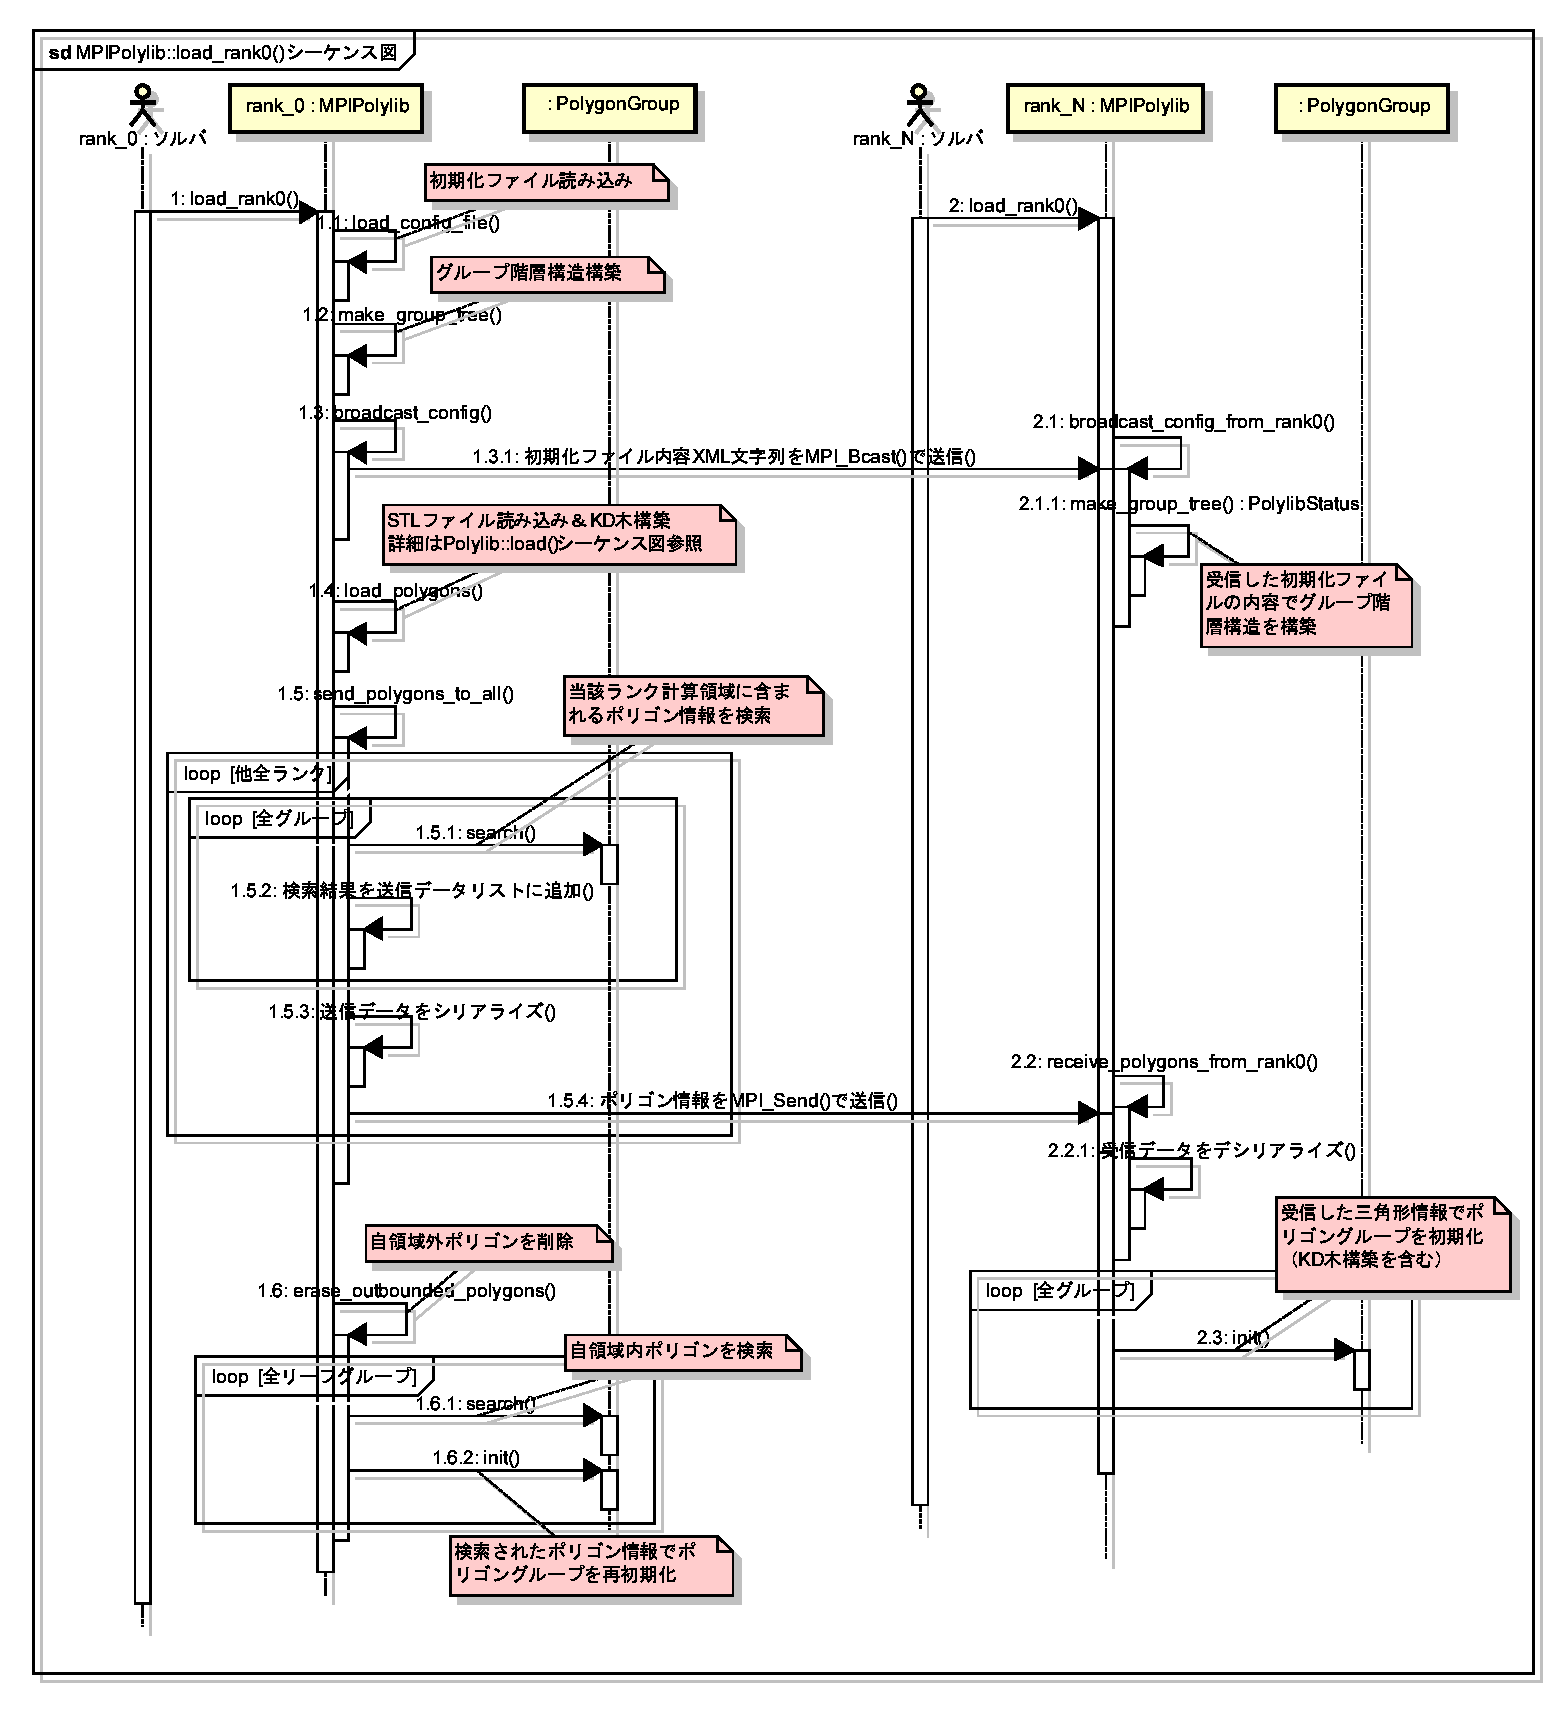
\includegraphics[width=16cm]{clip017.eps}
\end{figure}


\pagebreak
%
\subsection{MPIPolylib::load\_parallel()の内部処理シーケンス}

\begin{figure}[H]
 \centering
 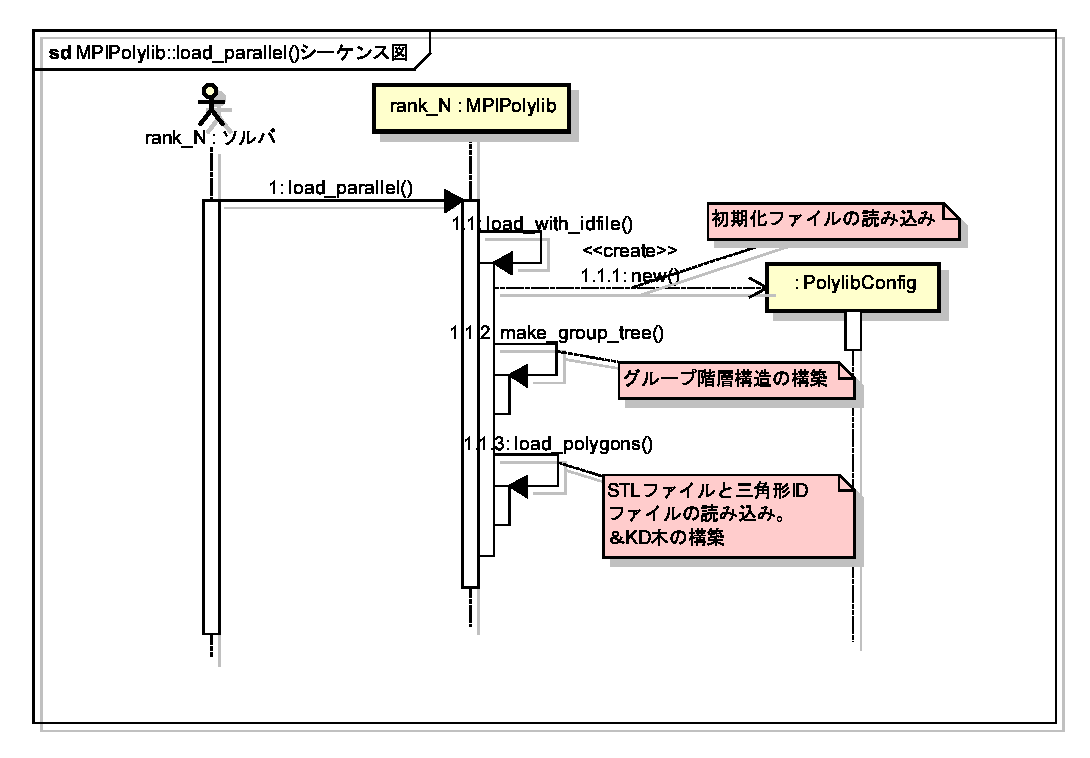
\includegraphics[width=13cm]{clip018.eps}
\end{figure}

%
\subsection{MPIPolylib::move()の内部処理シーケンス}

\begin{figure}[H]
 \centering
 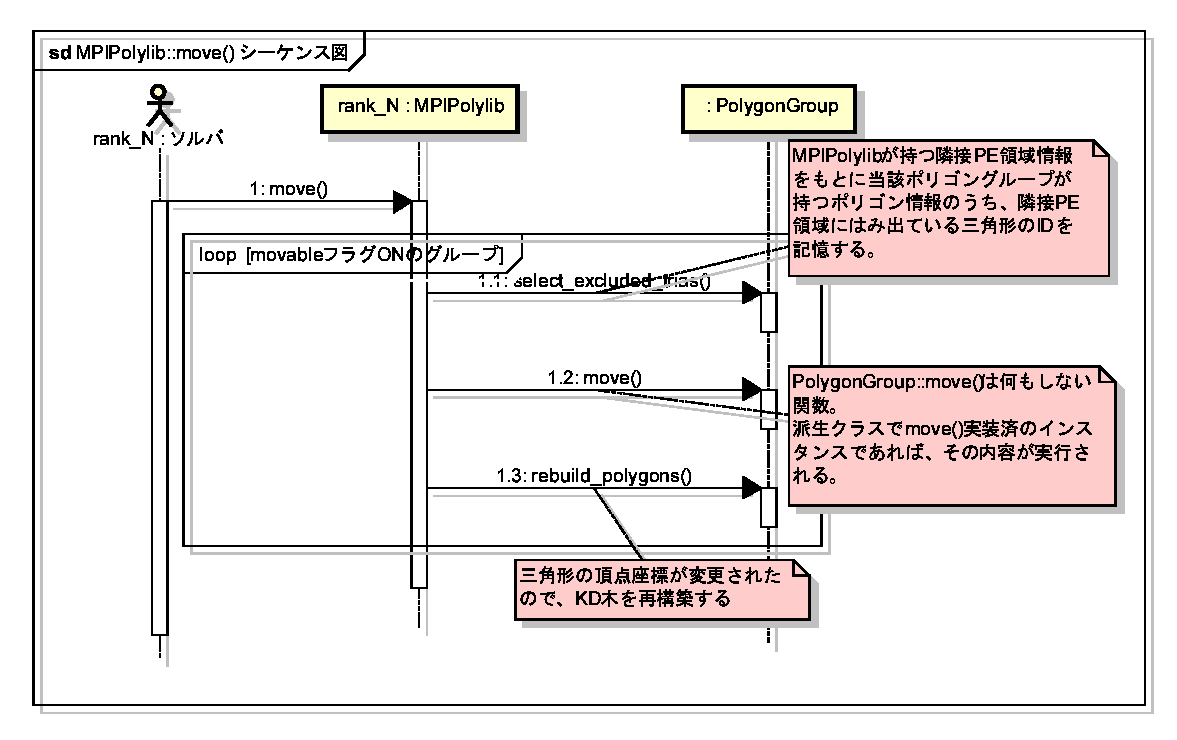
\includegraphics[width=13cm]{clip019.eps}
\end{figure}


\pagebreak
%
\subsection{MPIPolylib::migrate()の内部処理シーケンス}

\begin{figure}[H]
 \centering
 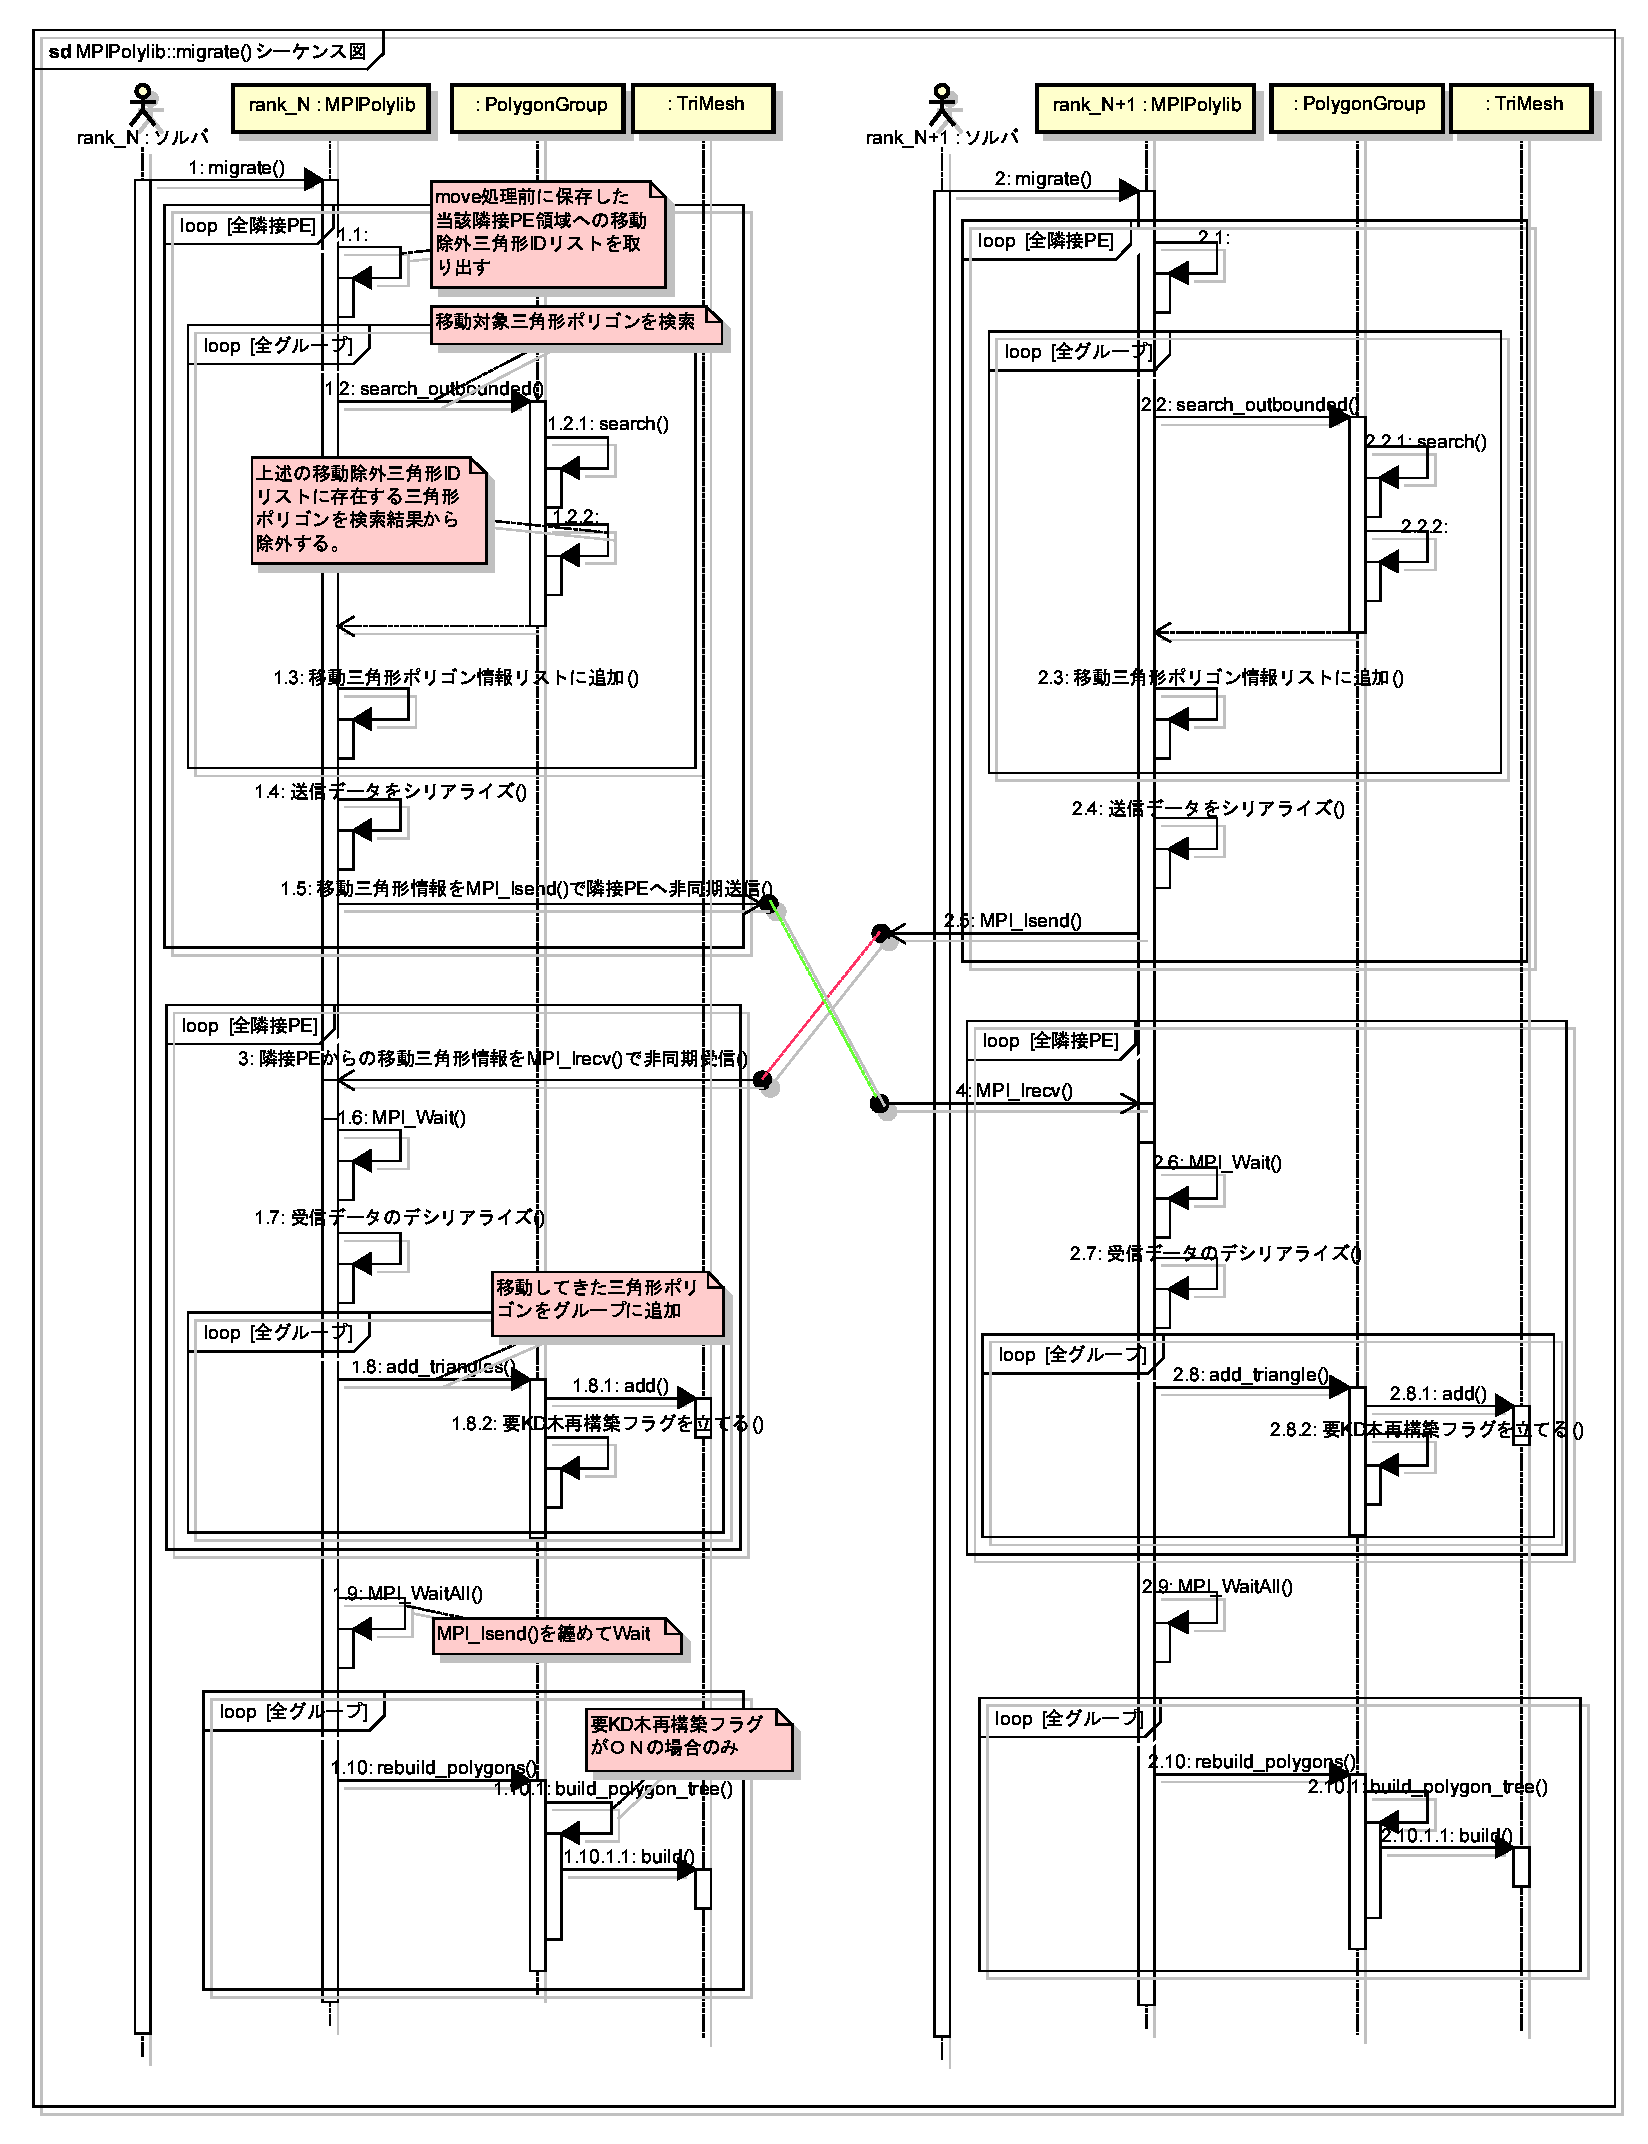
\includegraphics[width=16cm]{clip020.eps}
\end{figure}


\pagebreak
%
\subsection{MPIPolylib::save\_rank0()の内部処理シーケンス}

\begin{figure}[H]
 \centering
 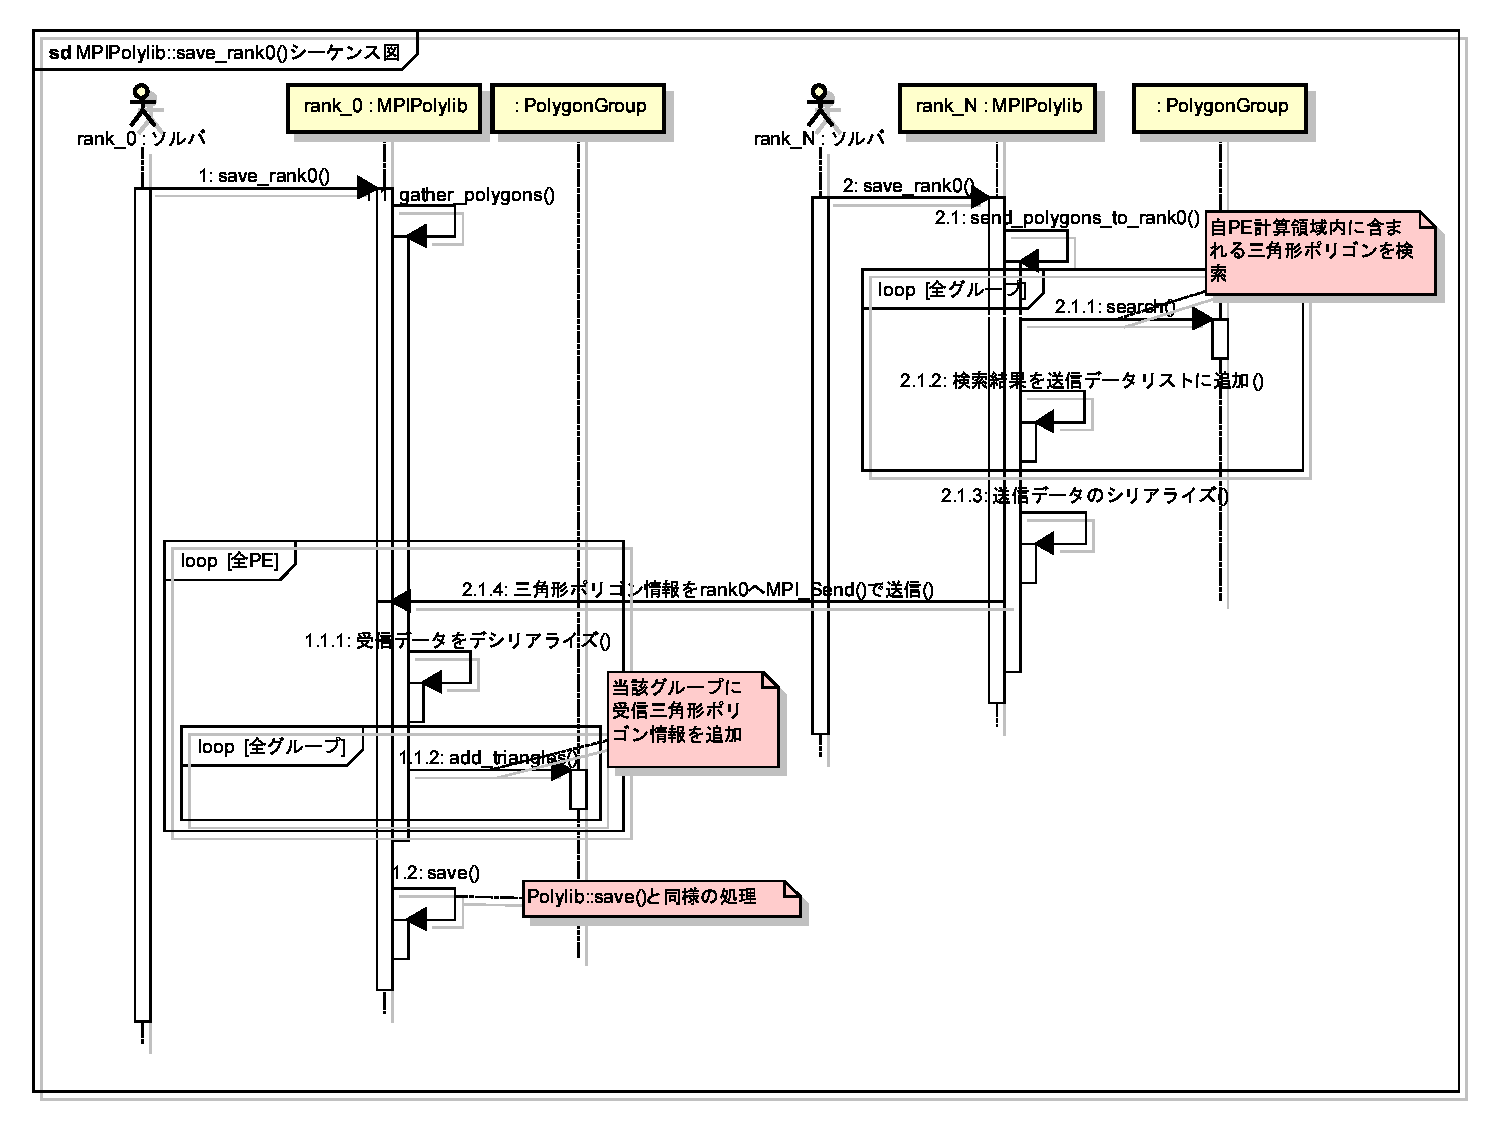
\includegraphics[width=16cm]{clip021.eps}
\end{figure}


\pagebreak
%
\subsection{MPIPolylib::save\_parallel()の内部処理シーケンス}

\begin{figure}[H]
 \centering
 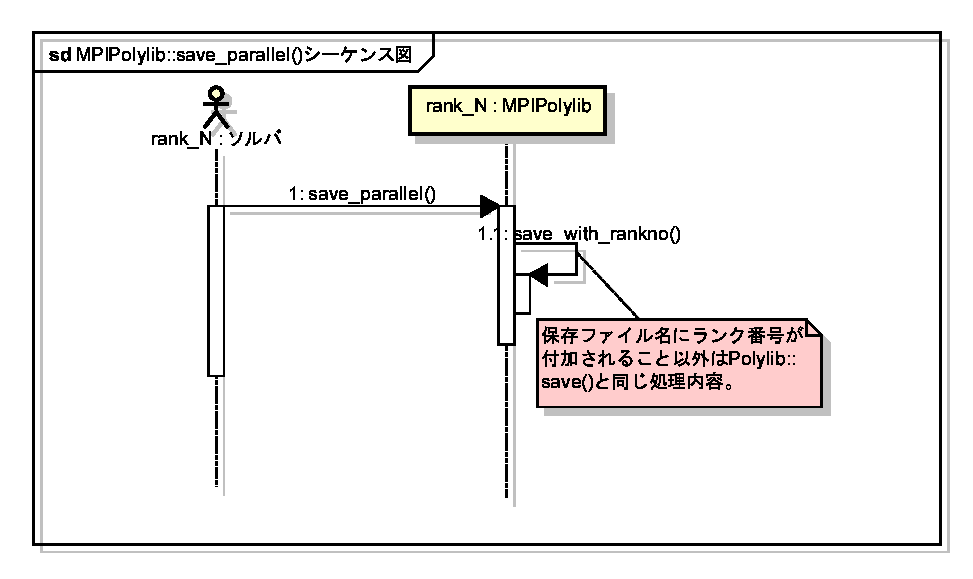
\includegraphics[width=12cm]{clip022.eps}
\end{figure}


\pagebreak
%
\subsection{(参考)MPIPolylibにおけるポリゴンの動的登録に関する検討結果}

Polylib Ver.2.0では,動的なポリゴングループの追加や削除に対応していません.これは開発時点
でその必要性について検討段階であったためです.

以下UMLシーケンス図はソルバー実行中にVOFLibにより新たにポリゴン情報が生成され,それを
MPIPolylibに登録した際の内部処理案です.

\begin{figure}[H]
 \centering
 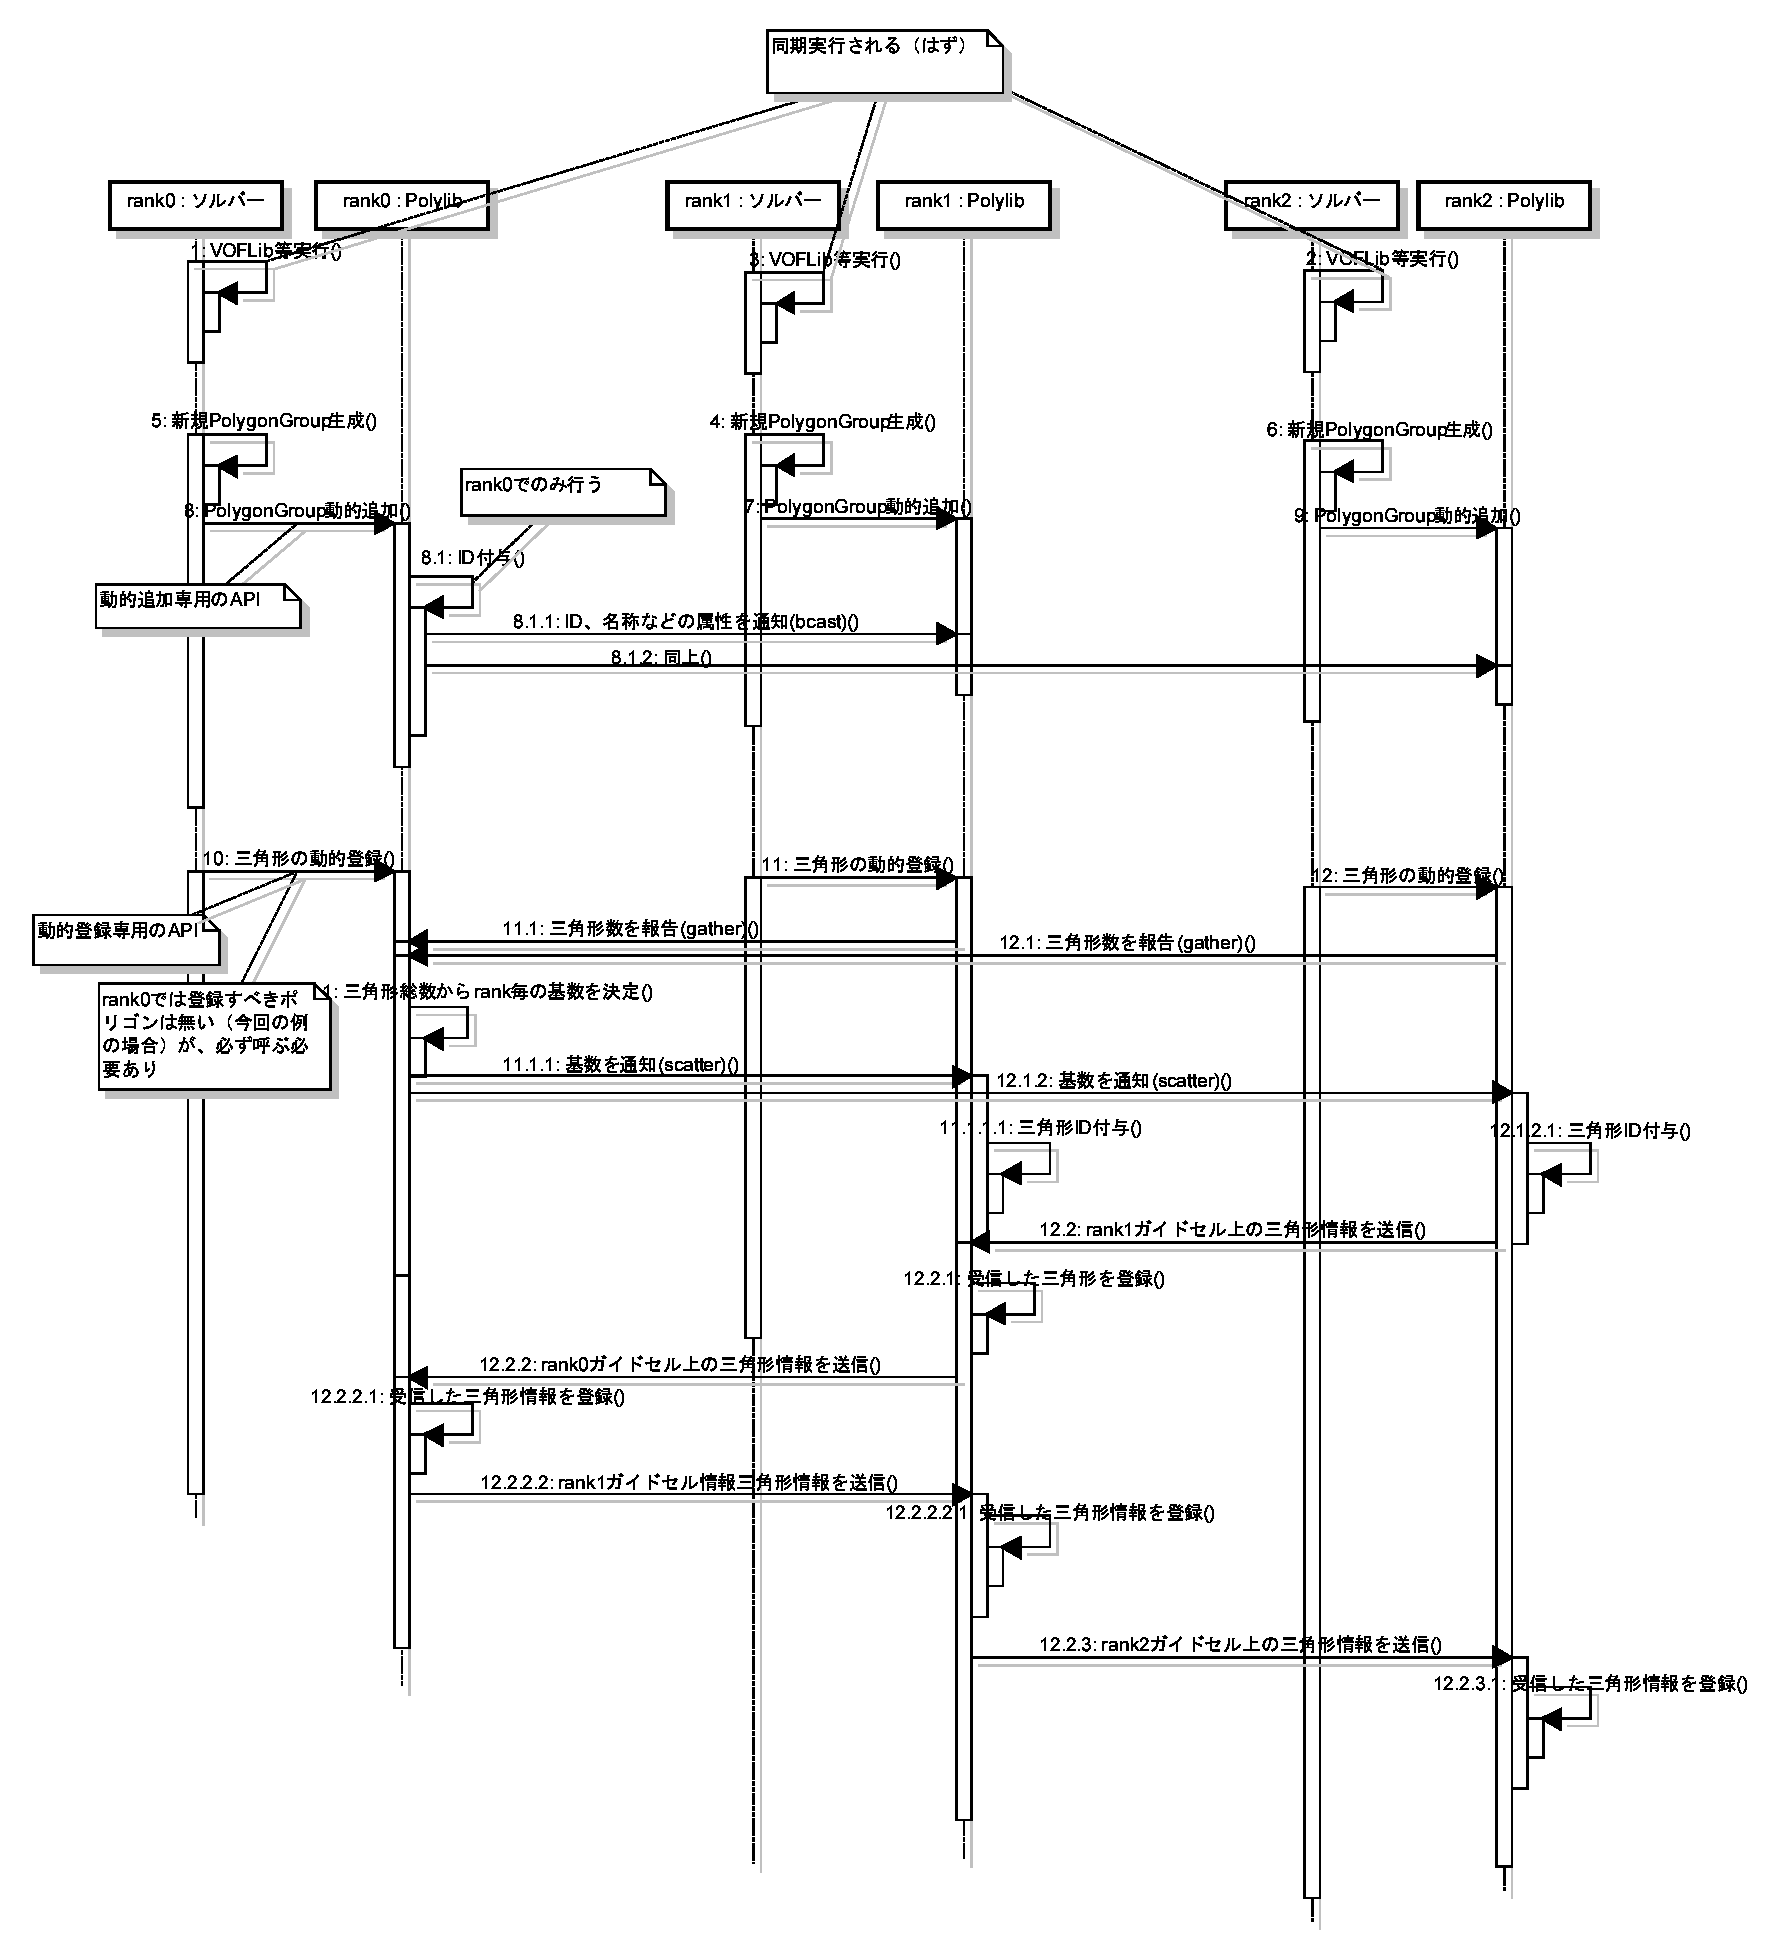
\includegraphics[width=16cm]{clip023.eps}
\end{figure}


\chapter{アップデート情報}
\begin{abstract}
本ユーザガイドのアップデート情報について記します.
\end{abstract}

%
\section{アップデート情報}

\begin{itemize}
	\item Version 2.0.3      22 Apr. 2012
	\begin{itemize}
		\item MPIPolylib::save\_parallel()で引数extendが指定されない場合、出力ファイル名に日付が付与されない不具合を修正
		\item PolygonGroup::get\_group\_area( void ), PolygonGroup::get\_group\_num\_tria( void )を追加
	\end{itemize}
\vspace{3mm}

	\item Version 2.0.2       5 Nov. 2010
	\begin{itemize}
		\item MPIPolylib::save\_parallel()およびload\_parallel()に引数id\_formatを追加.三角形IDファイルの形式をユーザプログラム側で選択可能とした
	\end{itemize}
\vspace{3mm}

	\item Version 2.0.1      29 Oct. 2010
	\begin{itemize}
		\item Polylib::get\_group( std::string )をpublicメソッドに変更
		\item Polylib::show\_group\_hierarchy()に引数FILE *fpを追加
		\item 三角形IDファイルについてバイナリ形式での入出力に対応
		\item 自ランク内に三角形ポリゴンを持たないPolygonGroupについてはSTLファイル・三角形IDファイルを出力しないこととした
		\item 初期化ファイルParamタグにユーザ定義id属性を設定可能にした
	\end{itemize}
\vspace{3mm}

	\item Version 2.0.0      30 Jul. 2010
	\begin{itemize}
		\item XML形式初期化ファイルに対応
		\item マイグレート機能を追加
		\item ポリゴン座標移動機能を追加
		\item ポリゴンデータの保存,再読み込み機能を追加
	\end{itemize}

\vspace{3mm}

	\item Version 1.0      26 Feb. 2010
	\begin{itemize}
		\item 初版リリース
	\end{itemize}
\end{itemize}

%
%\bibliographystyle{junsrt}
%\bibliography{cbc_UG}

\newpage
\printindex
%
%
\end{document}